\documentclass{tufte-handout}\usepackage[]{graphicx}\usepackage[]{xcolor}
% maxwidth is the original width if it is less than linewidth
% otherwise use linewidth (to make sure the graphics do not exceed the margin)
\makeatletter
\def\maxwidth{ %
  \ifdim\Gin@nat@width>\linewidth
    \linewidth
  \else
    \Gin@nat@width
  \fi
}
\makeatother

\definecolor{fgcolor}{rgb}{0.345, 0.345, 0.345}
\newcommand{\hlnum}[1]{\textcolor[rgb]{0.686,0.059,0.569}{#1}}%
\newcommand{\hlstr}[1]{\textcolor[rgb]{0.192,0.494,0.8}{#1}}%
\newcommand{\hlcom}[1]{\textcolor[rgb]{0.678,0.584,0.686}{\textit{#1}}}%
\newcommand{\hlopt}[1]{\textcolor[rgb]{0,0,0}{#1}}%
\newcommand{\hlstd}[1]{\textcolor[rgb]{0.345,0.345,0.345}{#1}}%
\newcommand{\hlkwa}[1]{\textcolor[rgb]{0.161,0.373,0.58}{\textbf{#1}}}%
\newcommand{\hlkwb}[1]{\textcolor[rgb]{0.69,0.353,0.396}{#1}}%
\newcommand{\hlkwc}[1]{\textcolor[rgb]{0.333,0.667,0.333}{#1}}%
\newcommand{\hlkwd}[1]{\textcolor[rgb]{0.737,0.353,0.396}{\textbf{#1}}}%
\let\hlipl\hlkwb

\usepackage{framed}
\makeatletter
\newenvironment{kframe}{%
 \def\at@end@of@kframe{}%
 \ifinner\ifhmode%
  \def\at@end@of@kframe{\end{minipage}}%
  \begin{minipage}{\columnwidth}%
 \fi\fi%
 \def\FrameCommand##1{\hskip\@totalleftmargin \hskip-\fboxsep
 \colorbox{shadecolor}{##1}\hskip-\fboxsep
     % There is no \\@totalrightmargin, so:
     \hskip-\linewidth \hskip-\@totalleftmargin \hskip\columnwidth}%
 \MakeFramed {\advance\hsize-\width
   \@totalleftmargin\z@ \linewidth\hsize
   \@setminipage}}%
 {\par\unskip\endMakeFramed%
 \at@end@of@kframe}
\makeatother

\definecolor{shadecolor}{rgb}{.97, .97, .97}
\definecolor{messagecolor}{rgb}{0, 0, 0}
\definecolor{warningcolor}{rgb}{1, 0, 1}
\definecolor{errorcolor}{rgb}{1, 0, 0}
\newenvironment{knitrout}{}{} % an empty environment to be redefined in TeX

\usepackage{alltt}

%\geometry{showframe}% for debugging purposes -- displays the margins

\usepackage{amsmath}
\usepackage{graphicx}
\usepackage{natbib}
\usepackage{cancel}
\usepackage{comment}

\setkeys{Gin}{width=\linewidth,totalheight=\textheight,keepaspectratio}
\bibfont{\small} % Doesn't see to work...

\graphicspath{{graphics/}}

\newenvironment{itemize*}%
  {\begin{itemize}%
    \setlength{\itemsep}{0pt}%
    \setlength{\parskip}{0pt}}%
  {\end{itemize}}
	
\newenvironment{enumerate*}%
  {\begin{enumerate}%
    \setlength{\itemsep}{0pt}%
    \setlength{\parskip}{0pt}}%
  {\end{enumerate}}
	
	\newenvironment{description*}%
  {\begin{description}%
    \setlength{\itemsep}{0pt}%
    \setlength{\parskip}{0pt}}%
  {\end{description}}

\newcommand{\numolspercm}{$\mu$mols/cm$^{-3}$}

\title{DRAFT! Advection, Diffusion \& Reaction Modeling}
\author{Marc Los Huertos}
\date{\today~(ver.~0.81)}

\setsidenotefont{\color{blue}}
% \setcaptionfont{hfont commandsi}
% \setmarginnotefont{\color{blue}}
% \setcitationfont{\color{gray}}

% The following package makes prettier tables.  We're all about the bling!
\usepackage{booktabs}

% Small sections of multiple columns
\usepackage{multicol}
\IfFileExists{upquote.sty}{\usepackage{upquote}}{}
\begin{document}

\maketitle% this prints the handout title, author, and date
\begin{abstract}
The movement of compounds in the environment is driven by two processes, advection and diffusion. The compounds are also subject to transformations or reactions. Thus, to monitor the fate and transport of compounds in the environment, we can capitalize on mathematical models that have been used to describe advection, diffusion, and reaction. %We'll begin with simple examples and then consider more complicated examples. We'll also consider the implications of these processes on the environment and human health.

%\sidenote{Typeset using the Sweave function in R and \LaTeX\ using a \citet{Tufte:1983, Tufte:1997} and style.}
\end{abstract}

\section{Introduction}

\subsection{Fate and Transport Processes}

The fate and transport of compounds in the environment is subject to an array of processes. For example, pollutants might carried by the wind (advection) and spread out (dispersion or diffusion). In addition, the pollutant might be transformed into different compounds (reaction). Together, these three processes, advection, diffusion, and reaction (Figure~\ref{fig:advection-diffusion}).%, can be effectively described mathematically, which can then be tested.

%. Of course, these processes occur in three dimensions but we'll focus on 1D and 2D for this session. 

\begin{marginfigure}
\centering
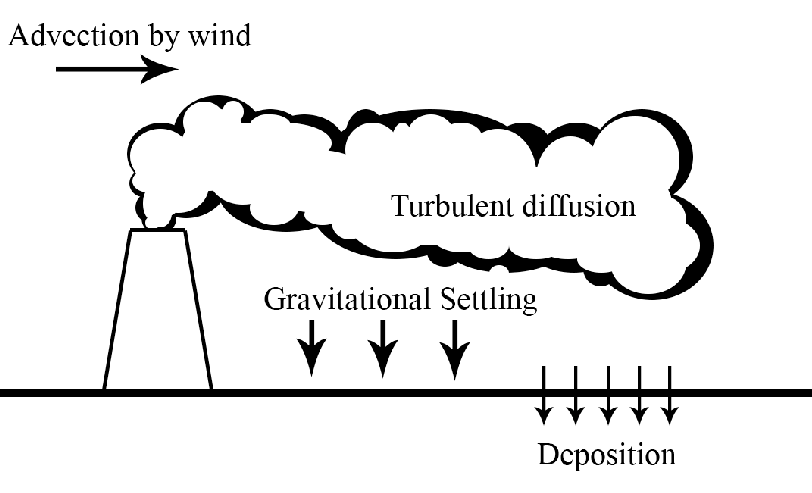
\includegraphics[width=1.0\textwidth]{graphics/Diagram-advection-diffusion.png}
\caption{A simple diagram of advection and diffusion that inclues how "solutes" might be deposited downwind of a stationary source if air pollution. At the scale analyzed there, the term turbulant diffusion is different than molecular diffusion, but might be modelled in a similar way.}
\label{fig:advection-diffusion}
\end{marginfigure}


These three processes have profound  implications -- they provide the a framework to understand and quantify the fate and transport of pollutants in the environment (Figure~\ref{fig:dioxaneplume}), the movement of nutrients in the soil, and the movement of solutes in the human body. By understanding of these processes, we have tools to characterize environmental quality and its implications on human and non-human populations. Moreover, by modeling these processes, we can develop more effective policy, regulation, and mitigation strategies.

\begin{figure*}
\centering
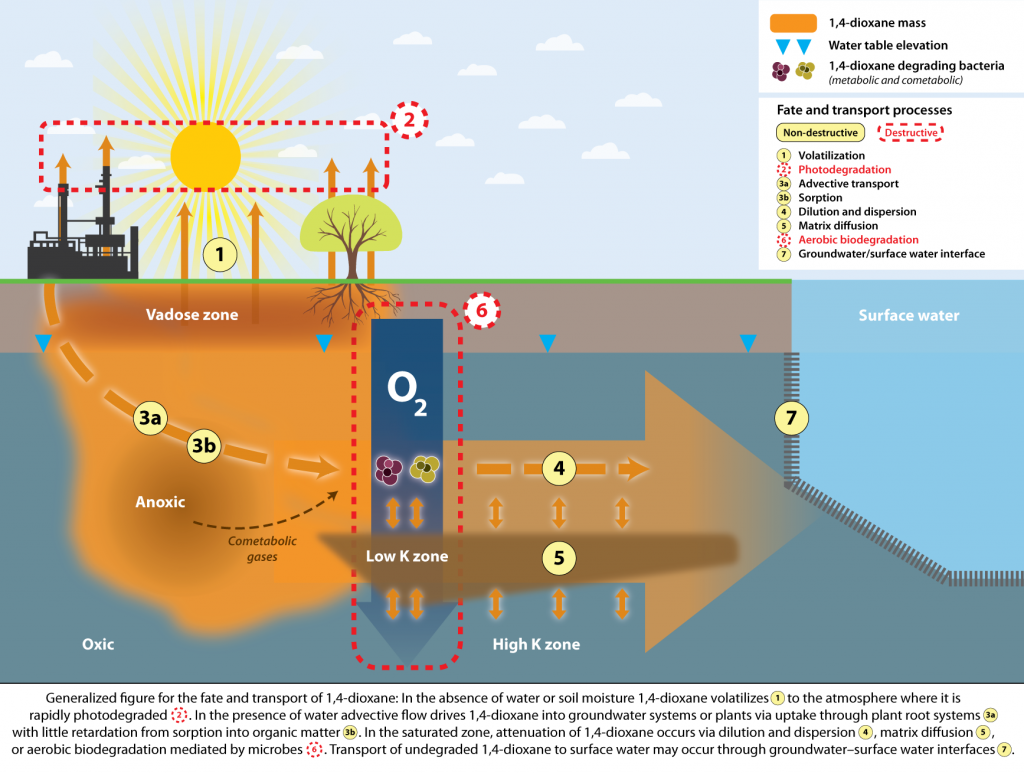
\includegraphics[width=0.9\textwidth]{graphics/Dioxane_plume.png}
\caption{A diagram of the major processes that influence the fate and transport of a dioxane plume from a ce in the environment (Source: \url{https://14d-1.itrcweb.org/environmental-fate-transport-and-investigative-strategies/}). 1,4-Dioxane is often referred to as a "forever" compound.}
\label{fig:dioxaneplume}
\end{figure*}

Because these processes are complex and are often difficult to measure, we rely on models to help us understand the movement of solutes in the environment. These models are based on the fundamental mathematical equations to describe advection, diffusion, and reaction.

\subsection{The Processes}

As an example of the three processes consider a droplet of dye in water as a dose in a solution. The dye will move with the bulk motion of the water (advection), spread out by random molecular motion (diffusion)(Figure~\ref{fig:diffusion}), and disappear as it reacts with the water (reaction).

Advection and diffusion govern the transport of solutes in the environment. Advection is the transport of a solute by the bulk motion of the fluid. Advection depends on velocity or $\nu$ in this session. Diffusion is the transport of a solute by random molecular motion. Diffusion depends on the diffusion coefficient and the concentration gradient or $\frac{\partial^2 C}{\partial x^2}$ in this session. Notice that this is the second derivative. 

\begin{marginfigure}
\caption{A simple diagram of 2D diffusion. To solve these equations, we'll use a numerical approach and descretize the media into a grid. We'll then solve the equations for each grid cell.}
\label{fig:diffusion}
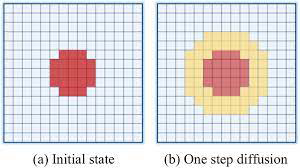
\includegraphics[width=1.0\textwidth]{graphics/2D_diffusion.png}
\end{marginfigure}

Reaction is the transformation of a solute into a different compound. Reaction depends on the reaction rate or $k$ in this session.

In the case of air pollution, we are interested in the pollutant in the context of the air -- or the media of air (Figure~\ref{fig:advection-diffusion}). And for air pollution, the chemical transormations are a critical part of our regulatory framework (Figure~\ref{}). In the case of water, we might think about solutes in the water as a media. For example, the movement of a nutrient in a river is driven by the bulk motion of the water (advection) through the water column and the sediments (two types of media) and the random motion of the molecules (diffusion) and the reactions that might occur in the water column and sediments (Figure\ref{fig:nutrientspiraling}).

\begin{figure*}
\caption{A simple diagram of advection and diffusion in the context of air pollution.}
\label{fig:smog}
\centering
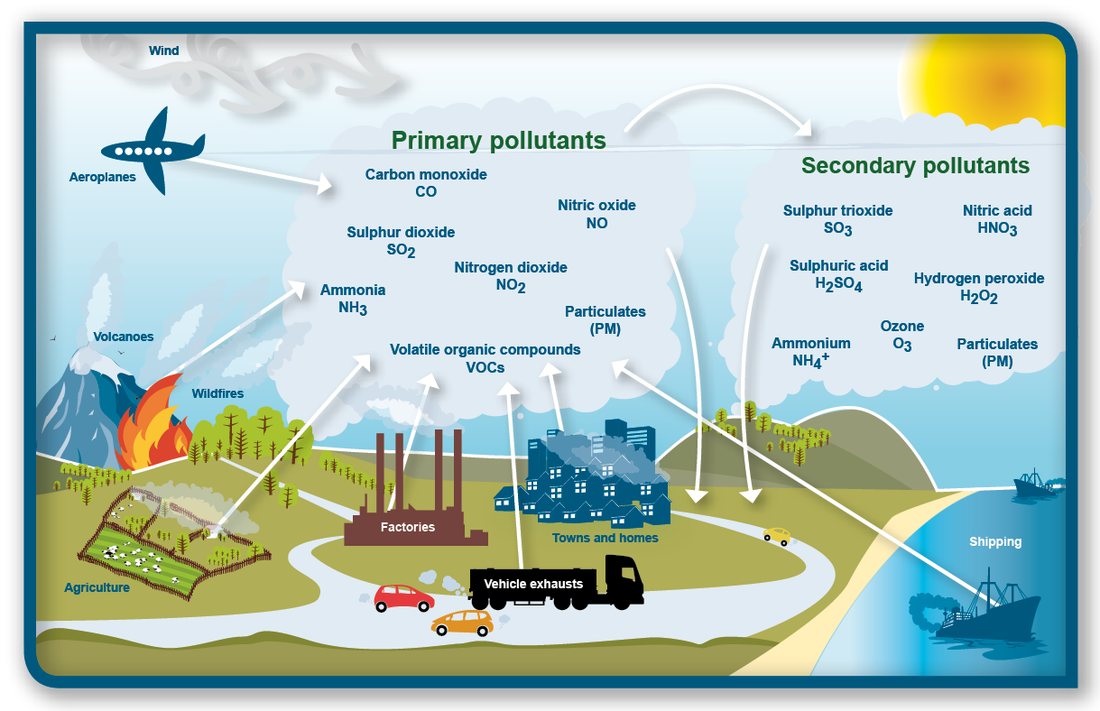
\includegraphics[width=0.99\textwidth]{graphics/sources-of-air-pollution-310314_orig.png}
\end{figure*}


\begin{figure}
\caption{A simple diagram of advection and nutrient reactions (organic substances and inorganic substances) in a river. Although not shown, you might also think about how diffusion might influence the movement of nutrients in the river and in the sediments.  
The zone where water moves into the sediment bed is called the hyperreic zone. The porosity of the sediments will allow more advective flow that might influence the reaction capacity of solutes in the sediments.}
\label{fig:nutrientspiraling}
\centering
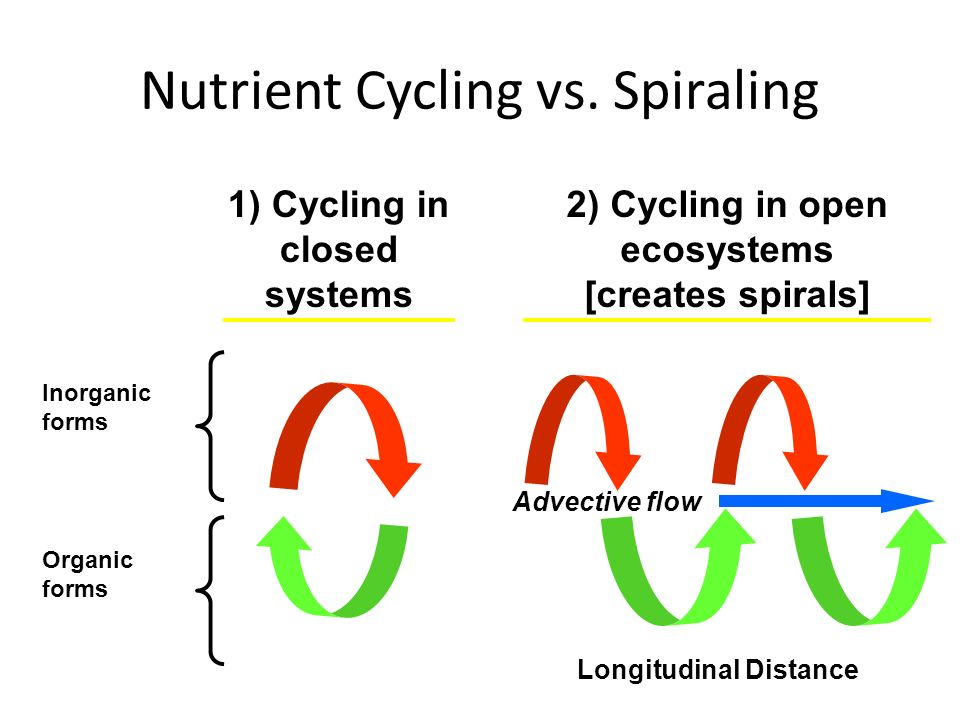
\includegraphics[width=0.99\textwidth]{graphics/NutrientSpiraling.jpg}
\end{figure}
jk
\subsection{Session Goals}

We will not become experts in advection-diffusion-reaction modeling, but we will become familiar with the processes and the equations that describe them. Moreover, we'll see a bit more about how R can be used to model these processes. After this session, I hope you can do the following:

\begin{enumerate*}
	\item Describe the physical processes of advection and diffusion and solute reaction
	\item Describe the equations used to model A-D-R. 
	\item Analyze 1-dimensional movement using advection equations in R.
	\item Describe diffusion mathematically
	\item Analyze 1-dimensional adveecton-diffusion using R.
	\item Appreciate how two-dimensional analysis of advection-diffusion can be modeled in R.
\end{enumerate*}

In this session, we'll want to think about the movement of solutes in the porous media, i.e. a soil with air space, sediments with water between the particles. We will refer to the porousity as $\xi$, which is a proportion between 0 and 1. 

\begin{marginfigure}
\centering
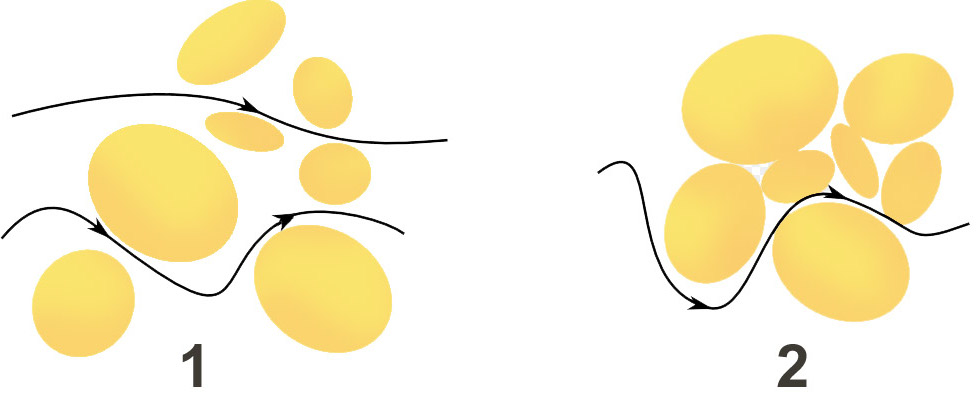
\includegraphics{graphics/Darcy_permeability.jpg}
\caption{Notice how the porosity of the media can influence the path of the fluid. In ground water, this is measured as permeability and can be used to evaluate the flow chacterstitics in aquifers and oil fields. The permeability is a function of the porosity and the connectivity of the pores.}
\end{marginfigure}

%We'll start with one-dimensional systems and then move to two-dimensional systems. We'll also consider the effects of reactions on the movement of solutes.

\section{Equations to Describe Processes}

\newthought{An Equation that Often Creates Anxiety}

The advection equation is a partial differential equation that describes the movement of a substance in a fluid. The equation is derived from the conservation of mass. The equation is:

%− 1 Axξx ·( ∂ ∂xAx·(−D· ∂ξxC ∂x )− ∂ ∂x(Ax·v·ξxC)) 

\begin{equation}
- \frac{1}{A_x \xi_x} \cdot \left( \frac{\partial}{\partial x} A_x \cdot \left( -D \cdot \frac{\partial \xi_x C}{\partial x} \right) - \frac{\partial}{\partial x} \left( A_x \cdot v \cdot \xi_x C \right) \right)
\end{equation}

\begin{equation}
\frac{\partial C}{\partial t} = D_x \frac{partial^2 C}{partial x^2} +
D_y \frac{\partial^2 C}{\partial y^2} +
D_z \frac{\partial^2 C}{\partial z^2} -
v_x \frac{\partial C}{\partial x} -
\lambda RC
\end{equation}

Here $D$ is the ``diffusion coefficient'', $\nu$ is the ``advection rate'' (or velocity), and $A_x$ and $\xi$ are the surface area and volume fraction, respectively.

As you complete the first part of this handout, please do some reflecting: 

\begin{quote}

What you look at this equation, think about how it makes you feel. It's a bit intimidating, to say the least. But that's only part of the story. I believe these equations, when put in front of is generates anxiety -- and this anxiety can be a barrier to learning. While it's easy to claim we can just put this anxiety away seems to be be a disservice and acknoweldgement of our emotional responses. Before moving forward, let's take a moment to acknowledge the anxiety and see where in your body you are feeling that. Take a deep breath and let it out several times before moving forward.

\end{quote} 

First, let's simplify this to 1-D (in one direction, x).

\begin{equation}
\frac{\partial C}{\partial t} = D \frac{\partial^2 C}{\partial x^2} - \nu \frac{\partial C}{\partial x} - R
\end{equation}

\subsection{Left side: $\frac{\partial C}{\partial t}$}

The left side of the equation describes the change in concentration over time. This is the rate of change of the concentration of the solute in the fluid. In steady state, this term is zero, which will use use to model the steady state concentration of the solute in the fluid.

\subsection{First term on the right side: $D \frac{\partial^2 C}{\partial x^2}$}

The first term on the right side of the equation describes the movement of the solute due to diffusion. This is the rate of change of the concentration of the solute in the fluid due to the movement of the solute from areas of high concentration to areas of low concentration.

\subsection{Second term on the right side: $- \nu \frac{\partial C}{\partial x}$}

The second term on the right side of the equation describes the movement of the solute due to advection. This is the rate of change of the concentration of the solute in the fluid due to the movement of the fluid.

\subsection{Third term on the right side: $- R$}

The third term on the right side of the equation describes the rate of change of the concentration of the solute in the fluid due to reactions. This is the rate of change of the concentration of the solute in the fluid due to the reaction of the solute with other compounds in the fluid.

\begin{quote}
\textbf{Pause for a moment:} Reflect on your emotional state. What are you feeling? Where are you feeling it? Take a deep breath and let it out several times. You have completed the reading for Wednesday's class.
\end{quote}

\section{Quatifying Advective Transport}

\begin{equation}
  J = C \cdot \nu
\end{equation}

J is the ``flux density'' of the solute, which is the amount of solute that moves through a unit area in a unit time. With units of $mass / (area \cdot time)$, the equation returns the rate of movement of the solute in the fluid.


We can take the derivative of the flux density with respect to the distance to get the ``flux rate'' and then derive the concentration change with respect to time: \sidenote{How dows J become C??}

\begin{equation}
  \frac{\partial J}{\partial x} = \nu \frac{\partial C}{\partial t}
\end{equation}


of the solute, which is the amount of solute that moves through a unit area in a unit time. With units of $mass / (area \cdot time)$, the equation returns the rate of movement of the solute in the fluid.

\section{Diffusion}

\subsection{Fick's First Law and Three Types of Diffusion}

There are three types of diffusion: turbulent (eddy) diffusion, dispersion and molecular diffusion. Each of the operate at different scales, but have similar effects and are describe by the same equation:

\begin{equation}\label{eq:ficks-first-law}
  J = -D \frac{d C}{dx}
\end{equation}

Equation~\ref{eq:ficks-first-law} ss known as Fick's first law. The negative sign indicates that the solute moves from areas of high concentration to areas of low concentration. The equation returns the rate of movement of the solute in the fluid.

\begin{description*}

\item[Turbulent or Eddy diffusion] is the movement of solutes due to the movement of the fluid. In this case, D is the ``eddy diffusion coefficient''.

\item[Dispersion] is the movement of solutes due to the random movement of the solute through a porous media where D is the ``dispersion coefficient''.

\item[Molecular diffusion] is the movement of solutes due to the random movement of the solute molecules where D is the ``molecular diffusion coefficient''.

\end{description*}

\subsection{Fick's Second Law -- Rate of Change}

Fick's Second Law is based on the conservation of mass, where the rate of change of the concentration of the solute in the fluid due to the movement of the solute from areas of high concentration to areas of low concentration is described by the equation:

\begin{equation}
  \frac{\partial C}{\partial t} = D \frac{\partial^2 C}{\partial x^2}
\end{equation}

which can be written as 

\begin{equation}
  \frac{\partial C}{\partial t} + D \frac{\partial^2 C}{\partial x^2} = 0
\end{equation}



We can rearrange Fick's first law to get the rate of change of the concentration of the solute in the fluid due to the movement of the solute from areas of high concentration to areas of low concentration:

\begin{equation}
  \frac{\partial C}{\partial t} + D \frac{\partial^2 C}{\partial x^2}
\end{equation}


Based on the conservation of mass, we can derive the rate of change of the concentration of the solute in the fluid due to the movement of the solute from areas of high concentration to areas of low concentration:


\begin{equation}
  \frac{\partial C}{\partial t} = D \frac{\partial^2 C}{\partial x^2}
\end{equation}

This equation is known as Fick's second law. It describes the rate of change of the concentration of the solute in the fluid due to the movement of the solute from areas of high concentration to areas of low concentration.


\section{Reaction}



\section{Setting Up Models in R}

\subsection{Grid and Time Step}


\subsection{Steady-state vs. Transient State}

\subsection{Boundary Conditions}

\subsection{Initial Conditions}

\subsection{Rate of Reaction}





\section{Implemeting Some 1D Examples in R}

\subsection{Plug Flow}

\subsection{Plug Flow through two media}


\subsection{Dissolved Oxygen Consumed in a Porous Media}

We will be modeling the consumption of oxygen in a "sand-sized" porous spherical particle. The model is based on the following equation:

\[ \frac{\partial C}{\partial t} = -v \frac{\partial C}{\partial x} - k(C) \]

where \( C \) is the concentration of oxygen, \( D \) is the diffusion coefficient, \( v \) is the velocity of the fluid, and \( k(C) \) is the rate of oxygen consumption.

At this scale the velocity will be zero. Thus, we will rely on diffusion to for the oxygen movement to where it is consumed. 



We start with defining the size and porosity of the particle and use R to create a grid to solve the advection-diffusion-reaction equation.

\begin{table}
\caption{Chararacteristics of the Particle}
\centering
\begin{tabular}{|l|l|c|c|} \hline
Parameter & Description & Typical Range &  Modelled Value \\ \hline\hline
\( R \) & Radius of the particle & \( 0.005-0.2 \) cm &  0.025 cm \\
Porosity & Proportion of void space & \(0.005-0.7\) &  0.7 \\ \hline
\end{tabular}
\end{table}

We will create a grid to model the particle with Radius \( R \) and \( N \) (= 100) grid points. We will also define the properties of the particle such as porosity, diffusion coefficient (D = 400), and the rate of oxygen consumption, R$_{02}$ = \ensuremath{10^{6}}.

Although we are modeling a one-dimensional system, we will need to create a grid surface as a circle to effectively model the particle surface area changes as O2 diffuses into the particle and is consumed by the reactions in the particle.

\begin{knitrout}
\definecolor{shadecolor}{rgb}{0.969, 0.969, 0.969}\color{fgcolor}\begin{kframe}
\begin{alltt}
\hlstd{grid} \hlkwb{<-} \hlkwd{setup.grid.1D}\hlstd{(}\hlkwc{x.up}\hlstd{=}\hlnum{0}\hlstd{,} \hlkwc{L} \hlstd{= R,} \hlkwc{N} \hlstd{= N)} \hlcom{# Grid definition}
\end{alltt}


{\ttfamily\noindent\bfseries\color{errorcolor}{\#\# Error in setup.grid.1D(x.up = 0, L = R, N = N): could not find function "{}setup.grid.1D"{}}}\begin{alltt}
\hlstd{por.grid} \hlkwb{<-} \hlkwd{setup.prop.1D}\hlstd{(}\hlkwc{value}\hlstd{=por,} \hlkwc{grid}\hlstd{=grid)} \hlcom{# Porosity}
\end{alltt}


{\ttfamily\noindent\bfseries\color{errorcolor}{\#\# Error in setup.prop.1D(value = por, grid = grid): could not find function "{}setup.prop.1D"{}}}\begin{alltt}
\hlstd{D.grid} \hlkwb{<-} \hlkwd{setup.prop.1D}\hlstd{(}\hlkwc{value}\hlstd{=D,} \hlkwc{grid}\hlstd{=grid)} \hlcom{# Diffusion coefficient}
\end{alltt}


{\ttfamily\noindent\bfseries\color{errorcolor}{\#\# Error in setup.prop.1D(value = D, grid = grid): could not find function "{}setup.prop.1D"{}}}\begin{alltt}
\hlstd{sphere.surf} \hlkwb{<-} \hlkwa{function}\hlstd{(}\hlkwc{x}\hlstd{)} \hlnum{4}\hlopt{*}\hlstd{pi}\hlopt{*}\hlstd{x}\hlopt{^}\hlnum{2} \hlcom{# Surface area of a sphere}
\hlstd{A.grid} \hlkwb{<-} \hlkwd{setup.prop.1D}\hlstd{(}\hlkwc{func}\hlstd{=sphere.surf,}  \hlkwc{grid}\hlstd{=grid)} \hlcom{# Surface area}
\end{alltt}


{\ttfamily\noindent\bfseries\color{errorcolor}{\#\# Error in setup.prop.1D(func = sphere.surf, grid = grid): could not find function "{}setup.prop.1D"{}}}\end{kframe}
\end{knitrout}

Finally, we need to define the O2 concentration at the surface of the particle and the O2 consumption rate of the particle. 

\begin{table}
\caption{Oxygen Consumption in the Particle}
\centering
\begin{tabular}{|l|l|c|c|} \hline
Parameter & Description & Typical Range &  Modelled Value \\ \hline\hline
\( C_{ow} \) & Concentration of O2 in Water & \( 0.1 - 0.3 \) \numolspercm &  0.25 \numolspercm \\
\( R_{02} \) & Rate of oxygen consumption & \( 10^5 - 10^6 \) \numolspercm~/year &  \ensuremath{10^{6}} \numolspercm/year \\
\( K_s \) & O2 saturation & \( 0.001 - 0.01 \) \numolspercm &  0.005 \numolspercm \\ \hline
\end{tabular}
\end{table}

Note, we often measure oxygen using ppm (parts per million), but the model uses \numolspercm. The conversion is 1 ppm = 0.0224 \numolspercm, thus, we are modeling \(Ks \) within a range of 2.24 - 6.72 ppm, using Ks = 0.22 \numolspercm.


Next we create a function to model the oxygen consumption in the, particle that relies on We will use the \texttt{tran.1D} function to solve the advection-diffusion equation and the \texttt{steady.1D} function to solve the steady state solution of the advection-diffusion-reaction equation.

\begin{knitrout}
\definecolor{shadecolor}{rgb}{0.969, 0.969, 0.969}\color{fgcolor}\begin{kframe}
\begin{alltt}
\hlstd{Aggregate.Model} \hlkwb{<-} \hlkwa{function}\hlstd{(}\hlkwc{time}\hlstd{,} \hlkwc{O2}\hlstd{,} \hlkwc{pars}\hlstd{) \{}
  \hlstd{tran} \hlkwb{<-} \hlkwd{tran.1D}\hlstd{(}\hlkwc{C} \hlstd{= O2,} \hlkwc{C.down} \hlstd{= C.ow.02,} \hlkwc{D} \hlstd{= D.grid,}
          \hlkwc{A}\hlstd{=A.grid,} \hlkwc{VF} \hlstd{= por.grid,} \hlkwc{dx} \hlstd{= grid)}
    \hlstd{reac} \hlkwb{<-} \hlopt{-} \hlstd{R.02} \hlopt{*} \hlstd{(O2} \hlopt{/}\hlstd{(Ks} \hlopt{+} \hlstd{O2))}
    \hlkwd{return}\hlstd{(}\hlkwd{list}\hlstd{(}\hlkwc{dCdt}\hlstd{= tran}\hlopt{$}\hlstd{dC} \hlopt{+} \hlstd{reac,} \hlkwc{reac} \hlstd{= reac,}
                \hlkwc{flux.up}\hlstd{=tran}\hlopt{$}\hlstd{flux.up,} \hlkwc{flux.down}\hlstd{=tran}\hlopt{$}\hlstd{flux.down))}
\hlstd{\}}


\hlstd{O2.agg} \hlkwb{<-} \hlkwd{steady.1D}\hlstd{(}\hlkwc{y} \hlstd{=} \hlkwd{runif}\hlstd{(N),} \hlkwc{func}\hlstd{=Aggregate.Model,}
                    \hlkwc{nspec}\hlstd{=}\hlnum{1}\hlstd{,} \hlkwc{positive}\hlstd{=}\hlnum{TRUE}\hlstd{,} \hlkwc{atol} \hlstd{=} \hlnum{1e-10}\hlstd{)}
\end{alltt}


{\ttfamily\noindent\bfseries\color{errorcolor}{\#\# Error in steady.1D(y = runif(N), func = Aggregate.Model, nspec = 1, positive = TRUE, : could not find function "{}steady.1D"{}}}\end{kframe}
\end{knitrout}


\begin{figure}
\centering
\caption{Oxygen Consumption in a Porous Sphere}
\begin{knitrout}
\definecolor{shadecolor}{rgb}{0.969, 0.969, 0.969}\color{fgcolor}\begin{kframe}


{\ttfamily\noindent\bfseries\color{errorcolor}{\#\# Error in plot(O2.agg, grid = grid\$x.mid, xlab = "{}Distance to Center"{}, : object 'O2.agg' not found}}\end{kframe}
\end{knitrout}
\end{figure}

The plot shows the oxygen concentration in the particle. The concentration is highest at the surface and decreases as it moves into the particle. The concentration is zero at the center of the particle.

\begin{figure}
\begin{knitrout}
\definecolor{shadecolor}{rgb}{0.969, 0.969, 0.969}\color{fgcolor}\begin{kframe}


{\ttfamily\noindent\bfseries\color{errorcolor}{\#\# Error in quantile(O2.agg\$y, probs = prob): object 'O2.agg' not found}}

{\ttfamily\noindent\bfseries\color{errorcolor}{\#\# Error in eval(expr, envir, enclos): object 'O2.agg' not found}}

{\ttfamily\noindent\bfseries\color{errorcolor}{\#\# Error in as.list(c(n, red)): object 'len' not found}}

{\ttfamily\noindent\bfseries\color{errorcolor}{\#\# Error in grid\$x.mid: object of type 'closure' is not subsettable}}

{\ttfamily\noindent\bfseries\color{errorcolor}{\#\# Error in as.graphicsAnnot(labels): object 'quant' not found}}\end{kframe}
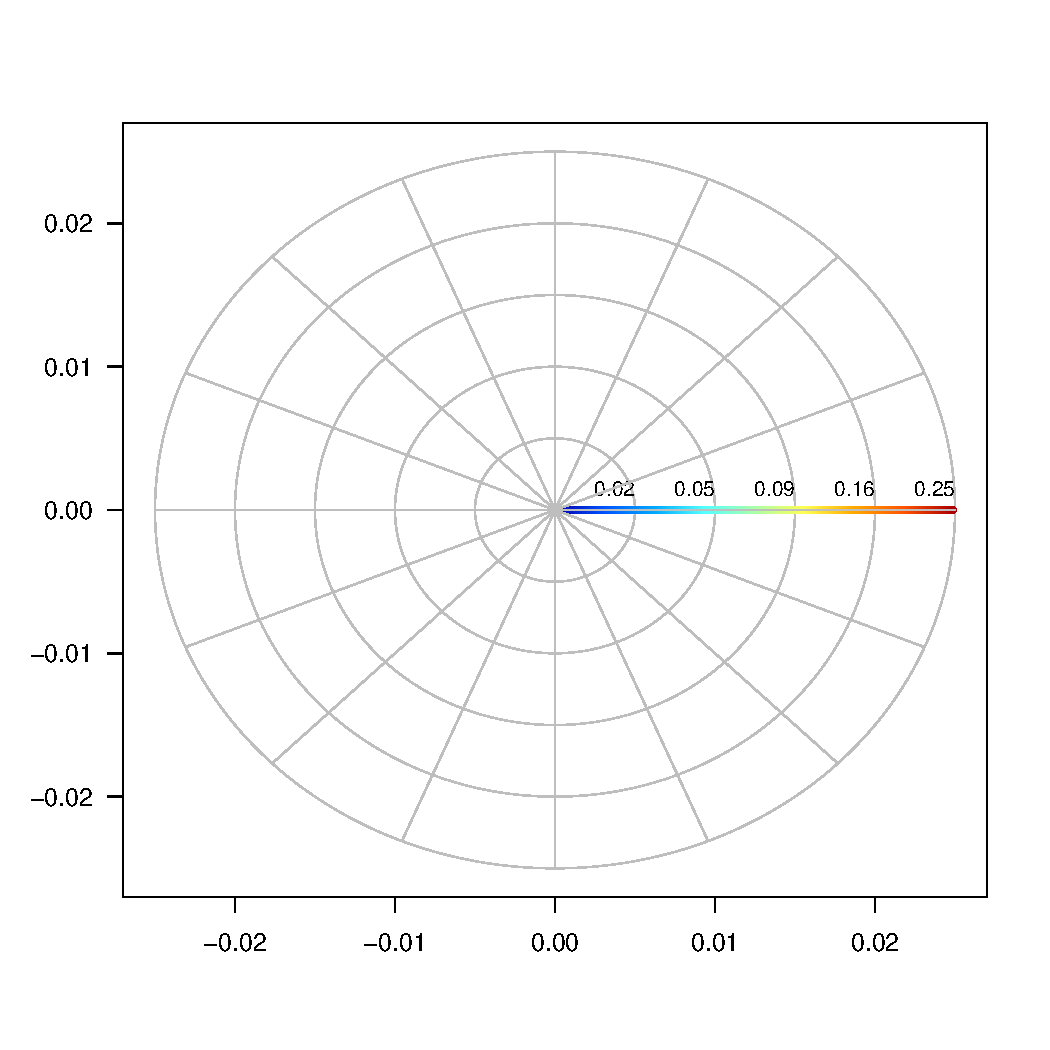
\includegraphics[width=\maxwidth]{figure/circleplot-1} 
\end{knitrout}
\end{figure}

Next steps: figure out how to create a 3D sphere with the oxygen concentration changes as we enter the sphere... 















\begin{comment}



Assuming that A, $\xi$, D and v are constant along x, we can rewrite this in a more general form: 

%D∂2C ∂x2−u∂C ∂x
\begin{equation}
\frac{\partial C/\partial t} =
D \frac{\partial^2 C}{\partial x^2} - \nu \frac{\partial C}{\partial x} - R
\end{equation}

where $\nu = v/A_x \xi_x$ is the ``velocity'' of the fluid.

The movement of compounds in the environment is driven by two processes, advection and diffusion. Of course, these processes occur in three dimensions, but for this class we'll begin with one dimensional processes before getting to more complicated examples.

Nevertheless, let's look at the 3-D advection-diffusion-reacton equation in three dimensions:

\begin{equation}
\frac{\partial C}{\partial t} = \nabla \cdot (D\nabla C - \nu C) + R
\end{equation}

where $C$ is the concentration of the solute, $t$ is time, $\nu$ is the velocity of the fluid, $D$ is the diffusion coefficient, and $R$ is the reaction term.

Ok, what what is $\nabla$? It's the gradient operator, which is a vector operator that operates on a scalar function to produce a vector whose magnitude is the maximum rate of change of the function at the point of the gradient and that points in the direction of that maximum rate of change. $\nabla \cdot$ represents divergence. In this equation, $\nabla C$ represents concentration gradient.

\subsection{Advection}

Advection is the process of transport of a solute by the bulk motion of the fluid. The rate of advection is proportional to the velocity of the fluid and the concentration of the solute. The rate of advection is given by the equation:

\begin{equation}
\frac{\partial C}{\partial t} + \nabla \cdot (\nu C) = 0
\end{equation}

where $C$ is the concentration of the solute, $t$ is time, and $\nu$ is the velocity of the fluid. 

For one dimensional systems, the equation can be written as:

\begin{equation}
\frac{\partial C}{\partial t} + \nu \frac{\partial C}{\partial x} = 0
\end{equation}

or

\begin{equation}
\frac{\partial C}{\partial t} + \nu_x \frac{\partial C}{\partial x}
\end{equation}

where $C$ is the concentration of the solute, $t$ is time, $\nu$ is the velocity of the fluid, and $x$ is the spatial coordinate.\sidenote{This can also be solved as a flux density -- the amount of solute that crosses a unit area per unit time, ${\displaystyle \mathbf {j} _{\text{adv}}=\mathbf {v} c}$.}


The advection equation is not simple to solve numerically: the system is a hyperbolic partial differential equation, and interest typically centers on discontinuous "shock" solutions (which are notoriously difficult for numerical schemes to handle).

T


\subsection{Diffusion}

Diffusion is the process of transport of a solute by random molecular motion. The rate of diffusion is proportional to the concentration gradient of the solute. The rate of diffusion is given by the equation:

\begin{equation}
\frac{\partial C}{\partial t} = D \nabla^2 C
\end{equation}

where $D$ is the diffusion coefficient.

\subsection{Advection-Diffusion Equation}

The advection-diffusion equation is a combination of the advection and diffusion equations. The advection-diffusion equation is given by the equation:

\begin{equation}
\frac{\partial C}{\partial t} + \nabla \cdot (\nu C) = D \nabla^2 C
\end{equation}

or 

\begin{equation}
\frac{\partial C}{\partial t} + u \frac{\partial C}{\partial x} = D \frac{\partial^2 C}{\partial x^2}
\end{equation}

where $C$ is the concentration of the solute, $t$ is time, $\nu$ is the velocity of the fluid, and $D$ is the diffusion coefficient.

\subsection{Advection-Difffusion-Reaction Equation}

The advection-diffusion-reaction equation is a combination the advection, diffusion, and reaction equations. The advection-diffusion-reaction equation is given by the equation:

\begin{equation}
\frac{\partial C}{\partial t} + \nabla \cdot (\nu C) = D \nabla^2 C + R
\end{equation}

where $C$ is the concentration of the solute, $t$ is time, $\nu$ is the velocity of the fluid, $D$ is the diffusion coefficient, and $R$ is the reaction term.

or in one-dimension:

\begin{equation}
\frac{\partial C}{\partial t} = \nu \frac{\partial C}{\partial x} = D \frac{\partial^2 C}{\partial x^2} + R
\end{equation}

where $C$ is the concentration of the solute, $t$ is time, $\nu$ is the velocity of the fluid, $D$ is the diffusion coefficient, and $R$ is the reaction term.

  
\subsection{Advenction-Difffusion-Reaction in multi-phase systems and for shapes with variable geometry}

The advection-diffusion-reaction equation can be extended to multi-phase systems and to shapes with variable geometry. The advection-diffusion-reaction equation for multi-phase systems and for shapes with variable geometry is given by the equation:

\begin{equation}
\frac{\partial C}{\partial t} + \nabla \cdot (\nu C) = D \nabla^2 C + R
\end{equation}

where $C$ is the concentration of the solute, $t$ is time, $\nu$ is the velocity of the fluid, $D$ is the diffusion coefficient, and $R$ is the reaction term.
  
\section{Applications using R}

\subsection{ReacTran Package}

\citet{soetaert2017package} have developed a nice library in R that solves these equations using finite-difference solutions. 

The ReacTran package is a collection of functions for modeling solute transport in 1D, 2D, and 3D. The package includes functions for solving the advection-diffusion equation, the advection-diffusion-reaction equation, and the advection-diffusion-reaction equation for multi-phase systems. 

The package also includes functions for solving:

\begin{itemize*}
\item Advection-diffusion equations in 1D, 2D, and 3D 
\item Advection-diffusion-reaction equations in 1D, 2D, and 3D
\item Advection-diffusion-reaction equations for multi-phase systems
\end{itemize*}

\subsection{Using R as a Modelling Environment to Solve PDEs and ODEs}

We can use R to solve the advection-diffusion equation. The `deSolve` package to solve the ReacTran library functions decomposing the partial differential equatation (PDE) into a descretized by space and solving be ordinary differential equations (ODE). 

\begin{knitrout}
\definecolor{shadecolor}{rgb}{0.969, 0.969, 0.969}\color{fgcolor}\begin{kframe}
\begin{alltt}
\hlkwd{library}\hlstd{(ReacTran)} \hlcom{# Load the ReacTran package}
\end{alltt}


{\ttfamily\noindent\itshape\color{messagecolor}{\#\# Loading required package: rootSolve}}

{\ttfamily\noindent\itshape\color{messagecolor}{\#\# Loading required package: deSolve}}

{\ttfamily\noindent\itshape\color{messagecolor}{\#\# Loading required package: shape}}\begin{alltt}
\hlkwd{library}\hlstd{(deSolve)} \hlcom{# Load the deSolve package}
\hlkwd{library}\hlstd{(xtable)} \hlcom{# Load the xtable package to help format tables outputs}
\end{alltt}
\end{kframe}
\end{knitrout}

\subsection{1D Transportion Model}

The `ReacTran` package provides a function to solve the advection-diffusion-reaction equation for a simple one-dimensional case.

\begin{knitrout}
\definecolor{shadecolor}{rgb}{0.969, 0.969, 0.969}\color{fgcolor}\begin{kframe}
\begin{alltt}
\hlkwd{tran.1D}\hlstd{(}\hlkwc{C} \hlstd{=} \hlnum{1}\hlstd{,} \hlkwc{D} \hlstd{=} \hlnum{0}\hlstd{,} \hlkwc{flux.up} \hlstd{=} \hlnum{1}\hlstd{,} \hlkwc{v} \hlstd{=} \hlnum{5}\hlstd{,} \hlkwc{A}\hlstd{=} \hlnum{1}\hlstd{,} \hlkwc{dx} \hlstd{=} \hlnum{1}\hlstd{,} \hlkwc{full.output} \hlstd{=} \hlnum{TRUE}\hlstd{)}
\end{alltt}
\begin{verbatim}
## $dC
## [1] -4
## 
## $C.up
## [1] 0.2
## 
## $C.down
## [1] 1
## 
## $dif.flux
## [1] 0 0
## 
## $adv.flux
## [1] 1 5
## 
## $flux
## [1] 1 5
## 
## $flux.up
## [1] 1
## 
## $flux.down
## [1] 5
\end{verbatim}
\end{kframe}
\end{knitrout}


\subsection{Solving a 1-D reaction tranport model}

\begin{knitrout}
\definecolor{shadecolor}{rgb}{0.969, 0.969, 0.969}\color{fgcolor}\begin{kframe}
\begin{alltt}
\hlkwd{library}\hlstd{(ReacTran)}
\hlstd{out} \hlkwb{<-} \hlkwd{steady.1D}\hlstd{(}\hlkwc{func} \hlstd{= advModel,} \hlkwc{y} \hlstd{=} \hlkwd{runif}\hlstd{(}\hlnum{25}\hlstd{),} \hlkwc{params} \hlstd{= parms,} \hlkwc{nspace}\hlstd{=} \hlnum{1}\hlstd{,} \hlkwc{positive} \hlstd{=} \hlnum{TRUE}\hlstd{)}
\end{alltt}
\end{kframe}
\end{knitrout}

We can use R to solve the advection-diffusion-reaction equation. The following code uses the `deSolve` package to solve the advection-diffusion-reaction equation for a simple one-dimensional case.

\begin{knitrout}
\definecolor{shadecolor}{rgb}{0.969, 0.969, 0.969}\color{fgcolor}\begin{kframe}
\begin{alltt}
\hlcom{# Load the deSolve package}
\hlkwd{library}\hlstd{(deSolve)}

\hlcom{# Define the advection-diffusion-reaction equation}
\hlstd{advection_diffusion_reaction} \hlkwb{<-} \hlkwa{function}\hlstd{(}\hlkwc{t}\hlstd{,} \hlkwc{C}\hlstd{,} \hlkwc{parms}\hlstd{) \{}
  \hlkwd{with}\hlstd{(}\hlkwd{as.list}\hlstd{(parms), \{}
    \hlstd{dC} \hlkwb{<-} \hlstd{D} \hlopt{*} \hlstd{(}\hlkwd{diff}\hlstd{(C,} \hlkwc{lag} \hlstd{=} \hlnum{2}\hlstd{)} \hlopt{-} \hlnum{2} \hlopt{*} \hlkwd{diff}\hlstd{(C,} \hlkwc{lag} \hlstd{=} \hlnum{1}\hlstd{)} \hlopt{+} \hlkwd{diff}\hlstd{(C,} \hlkwc{lag} \hlstd{=} \hlnum{0}\hlstd{))} \hlopt{/} \hlstd{dx}\hlopt{^}\hlnum{2} \hlopt{-} \hlstd{k} \hlopt{*} \hlstd{C}
    \hlstd{dC[}\hlnum{1}\hlstd{]} \hlkwb{<-} \hlnum{0}
    \hlstd{dC[n]} \hlkwb{<-} \hlnum{0}
    \hlkwd{list}\hlstd{(dC)}
  \hlstd{\})}
\hlstd{\}}

\hlcom{# Set the parameters}
\hlstd{parms} \hlkwb{<-} \hlkwd{list}\hlstd{(}
  \hlkwc{D} \hlstd{=} \hlnum{0.1}\hlstd{,}  \hlcom{# Diffusion coefficient}
  \hlkwc{dx} \hlstd{=} \hlnum{0.1}\hlstd{,}  \hlcom{# Spatial step}
  \hlkwc{k} \hlstd{=} \hlnum{0.01}  \hlcom{# Reaction rate}
\hlstd{)}

\hlcom{# Set the initial conditions}
\hlstd{C0} \hlkwb{<-} \hlkwd{c}\hlstd{(}\hlnum{0}\hlstd{,} \hlkwd{rep}\hlstd{(}\hlnum{0}\hlstd{,} \hlnum{98}\hlstd{),} \hlnum{1}\hlstd{,} \hlkwd{rep}\hlstd{(}\hlnum{0}\hlstd{,} \hlnum{98}\hlstd{),} \hlnum{0}\hlstd{)}

\hlcom{# Set the times at which to evaluate the solution}
\hlstd{times} \hlkwb{<-} \hlkwd{seq}\hlstd{(}\hlnum{0}\hlstd{,} \hlnum{100}\hlstd{,} \hlkwc{by} \hlstd{=} \hlnum{1}\hlstd{)}

\hlcom{# Solve the advection-diffusion-reaction equation}
\hlstd{out} \hlkwb{<-} \hlkwd{ode}\hlstd{(}\hlkwc{y} \hlstd{= C0,} \hlkwc{times} \hlstd{= times,} \hlkwc{func} \hlstd{= advection_diffusion_reaction,} \hlkwc{parms} \hlstd{= parms)}

\hlcom{# Plot the solution}
\hlkwd{plot}\hlstd{(out,} \hlkwc{xlab} \hlstd{=} \hlstr{"Distance"}\hlstd{,} \hlkwc{ylab} \hlstd{=} \hlstr{"Concentration"}\hlstd{,} \hlkwc{type} \hlstd{=} \hlstr{"l"}\hlstd{)}
\end{alltt}
\end{kframe}
\end{knitrout}

\subsection{1-D Reaction-Transport Model}

For this example, we will solve the advection-diffusion-reaction equation for a simple one-dimensional case, where the reaction term is given by $R = kC$, and the initial concentration is given by $C(x,0) = 1$ for $x < ?$ and $C(x,0) = 1$ for $x \geq 0.5$. 



% latex table generated in R 4.2.2 by xtable 1.8-4 package
% Wed Feb 21 07:17:12 2024
\begin{table}[ht]
\centering
\begin{tabular}{rr}
  \hline
 & Value \\ 
  \hline
F0 & 1.00 \\ 
  v & 1.00 \\ 
  k & 0.10 \\ 
  D & 0.00 \\ 
  dx & 1.00 \\ 
   \hline
\end{tabular}
\end{table}



\begin{knitrout}
\definecolor{shadecolor}{rgb}{0.969, 0.969, 0.969}\color{fgcolor}\begin{kframe}
\begin{alltt}
\hlstd{advModel} \hlkwb{<-} \hlkwa{function}\hlstd{(}\hlkwc{t}\hlstd{,} \hlkwc{C}\hlstd{,} \hlkwc{parms}\hlstd{) \{}
  \hlkwd{with}\hlstd{(}\hlkwd{as.list}\hlstd{(parms), \{}
    \hlstd{Tran} \hlkwb{<-} \hlkwd{tran.1D}\hlstd{(}\hlkwc{C} \hlstd{= C,} \hlkwc{D} \hlstd{= D,} \hlkwc{flux.up} \hlstd{= F0,} \hlkwc{v} \hlstd{= v,} \hlkwc{dx} \hlstd{= dx)}
    \hlstd{Consumption} \hlkwb{=} \hlstd{k} \hlopt{*} \hlstd{C}
    \hlstd{dC} \hlkwb{<-} \hlstd{Tran}\hlopt{$}\hlstd{dC} \hlopt{-} \hlstd{Consumption}

    \hlkwd{return}\hlstd{(}\hlkwd{list}\hlstd{(}\hlkwc{dC} \hlstd{= dC,} \hlkwc{Consumption} \hlstd{= Consumption,} \hlkwc{flux.up} \hlstd{= Tran}\hlopt{$}\hlstd{flux.up,} \hlkwc{flux.down} \hlstd{= Tran}\hlopt{$}\hlstd{flux.down))}
  \hlstd{\})}
\hlstd{\}}

\hlstd{out} \hlkwb{<-} \hlkwd{steady.1D}\hlstd{(}\hlkwc{func} \hlstd{= advModel,} \hlkwc{y} \hlstd{=} \hlkwd{runif}\hlstd{(}\hlnum{25}\hlstd{),} \hlkwc{parms} \hlstd{= parms,} \hlkwc{nspec}\hlstd{=} \hlnum{1}\hlstd{,} \hlkwc{positive} \hlstd{=} \hlnum{TRUE}\hlstd{)}

\hlstd{parms} \hlkwb{<-} \hlkwd{c}\hlstd{(}\hlkwc{F0} \hlstd{=} \hlnum{1}\hlstd{,} \hlkwc{v}\hlstd{=}\hlnum{1}\hlstd{,} \hlkwc{k} \hlstd{=} \hlnum{0.5}\hlstd{,} \hlkwc{D}\hlstd{=}\hlnum{0}\hlstd{,} \hlkwc{dx} \hlstd{=} \hlnum{1}\hlstd{)}
\hlstd{out2} \hlkwb{<-} \hlkwd{steady.1D}\hlstd{(}\hlkwc{func} \hlstd{= advModel,} \hlkwc{y} \hlstd{=} \hlkwd{runif}\hlstd{(}\hlnum{25}\hlstd{),} \hlkwc{parms} \hlstd{= parms,} \hlkwc{nspec}\hlstd{=} \hlnum{1}\hlstd{,} \hlkwc{positive} \hlstd{=} \hlnum{TRUE}\hlstd{)}

\hlstd{parms} \hlkwb{<-} \hlkwd{c}\hlstd{(}\hlkwc{F0} \hlstd{=} \hlnum{1}\hlstd{,} \hlkwc{v}\hlstd{=}\hlnum{1}\hlstd{,} \hlkwc{k} \hlstd{=} \hlnum{0.5}\hlstd{,} \hlkwc{D}\hlstd{=}\hlnum{50}\hlstd{,} \hlkwc{dx} \hlstd{=} \hlnum{1}\hlstd{)}
\hlstd{out3} \hlkwb{<-} \hlkwd{steady.1D}\hlstd{(}\hlkwc{func} \hlstd{= advModel,} \hlkwc{y} \hlstd{=} \hlkwd{runif}\hlstd{(}\hlnum{25}\hlstd{),} \hlkwc{parms} \hlstd{= parms,} \hlkwc{nspec}\hlstd{=} \hlnum{1}\hlstd{,} \hlkwc{positive} \hlstd{=} \hlnum{TRUE}\hlstd{)}
\end{alltt}
\end{kframe}
\end{knitrout}

We can look at the output, using a simple call of the object, but without more information, it's not clear what we are looking at. 
\begin{knitrout}
\definecolor{shadecolor}{rgb}{0.969, 0.969, 0.969}\color{fgcolor}\begin{kframe}
\begin{alltt}
\hlstd{out}
\end{alltt}
\begin{verbatim}
## $y
##  [1] 0.9090909 0.8264463 0.7513148 0.6830135 0.6209213 0.5644739 0.5131581
##  [8] 0.4665074 0.4240976 0.3855433 0.3504939 0.3186308 0.2896644 0.2633313
## [15] 0.2393921 0.2176291 0.1978447 0.1798588 0.1635080 0.1486436 0.1351306
## [22] 0.1228460 0.1116782 0.1015256 0.0922960
## 
## $Consumption
##  [1] 0.09090909 0.08264463 0.07513148 0.06830135 0.06209213 0.05644739
##  [7] 0.05131581 0.04665074 0.04240976 0.03855433 0.03504939 0.03186308
## [13] 0.02896644 0.02633313 0.02393921 0.02176291 0.01978447 0.01798588
## [19] 0.01635080 0.01486436 0.01351306 0.01228460 0.01116782 0.01015256
## [25] 0.00922960
## 
## $flux.up
## [1] 1
## 
## $flux.down
## [1] 0.092296
## 
## attr(,"precis")
## [1] 3.372309e-01 1.305650e-09
## attr(,"steady")
## [1] TRUE
## attr(,"class")
## [1] "steady1D"  "rootSolve" "list"     
## attr(,"dimens")
## [1] 25
## attr(,"nspec")
## [1] 1
\end{verbatim}
\end{kframe}
\end{knitrout}

Thus, we might be better off plotting the output. I am not sure why the plot functions are ignoring my par() call, perhaps this will be fixed by version 0.9!

\begin{figure*}
\begin{knitrout}
\definecolor{shadecolor}{rgb}{0.969, 0.969, 0.969}\color{fgcolor}
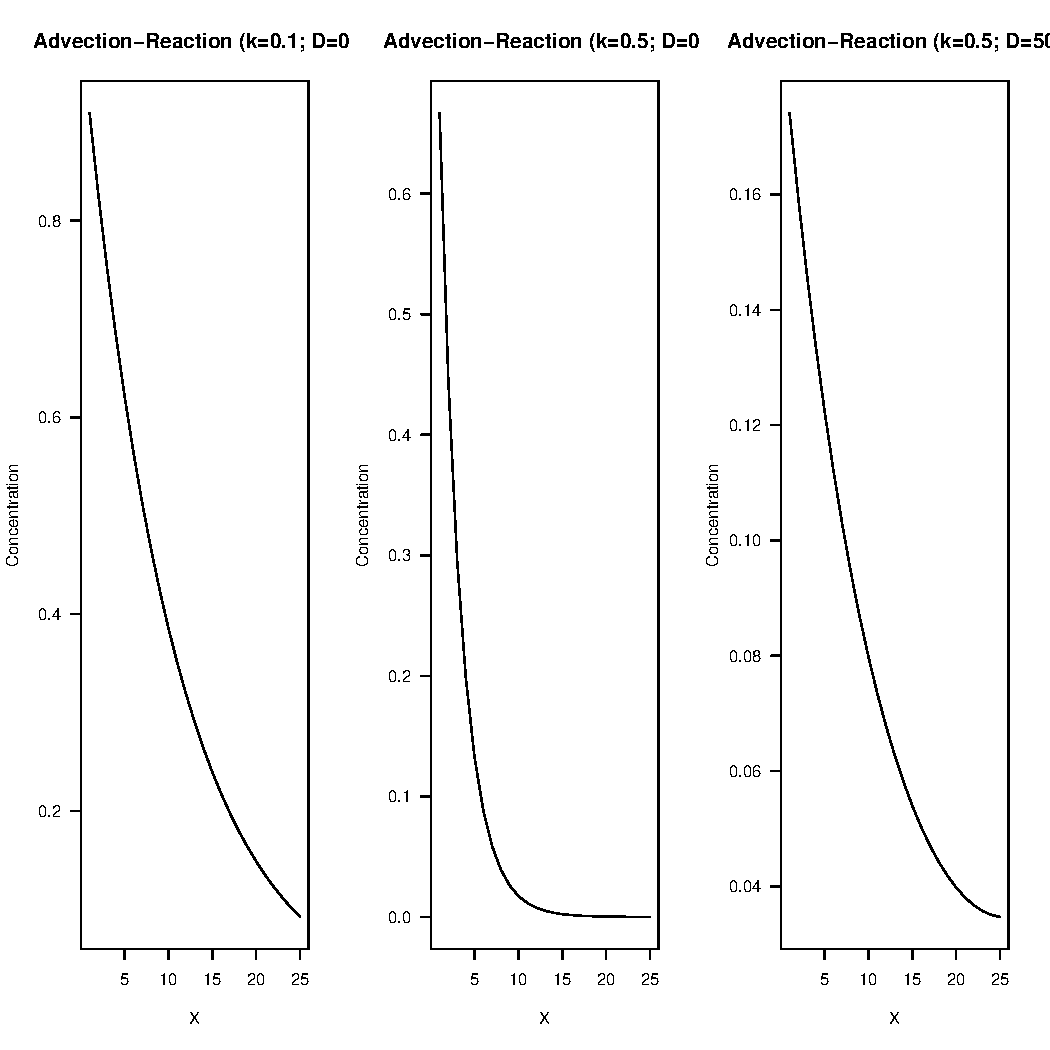
\includegraphics[width=4in,height=5in]{figure/1D-AdvectionReaction-1} 
\end{knitrout}
\end{figure*}

\subsection{asdf}

\begin{knitrout}
\definecolor{shadecolor}{rgb}{0.969, 0.969, 0.969}\color{fgcolor}\begin{kframe}
\begin{alltt}
\hlstd{Grid}\hlkwb{<-}\hlkwd{setup.grid.1D}\hlstd{(}\hlkwc{N}\hlstd{=}\hlnum{1000}\hlstd{,}\hlkwc{L}\hlstd{=}\hlnum{10}\hlstd{)}
\hlstd{r} \hlkwb{<-}\hlkwd{setup.prop.1D}\hlstd{(}\hlkwc{grid}\hlstd{=Grid,}\hlkwc{func}\hlstd{=}\hlkwa{function}\hlstd{(}\hlkwc{r}\hlstd{)r)}
\hlstd{r2}\hlkwb{<-}\hlkwd{setup.prop.1D}\hlstd{(}\hlkwc{grid}\hlstd{=Grid,}\hlkwc{func}\hlstd{=}\hlkwa{function}\hlstd{(}\hlkwc{r}\hlstd{)r}\hlopt{^}\hlnum{2}\hlstd{)}


\hlstd{pde1D}\hlkwb{<-}\hlkwa{function}\hlstd{(}\hlkwc{t}\hlstd{,}\hlkwc{C}\hlstd{,}\hlkwc{parms}\hlstd{,}\hlkwc{A}\hlstd{=}\hlnum{1}\hlstd{)\{}
  \hlstd{tran}\hlkwb{<-}\hlkwd{tran.1D}\hlstd{(}\hlkwc{C}\hlstd{=C,}\hlkwc{A}\hlstd{=A,}\hlkwc{D}\hlstd{=D,}\hlkwc{C.down}\hlstd{=Cext,} \hlkwc{dx}\hlstd{=Grid)}\hlopt{$}\hlstd{dC}
  \hlkwd{list}\hlstd{(tran}\hlopt{-}\hlstd{Q)}
\hlstd{\}}

\hlstd{D}\hlkwb{<-}\hlnum{1}
\hlstd{Q}\hlkwb{<-}\hlnum{1}
\hlstd{Cext}\hlkwb{<-}\hlnum{20}



\hlstd{Cartesian} \hlkwb{<-}\hlkwd{steady.1D}\hlstd{(}\hlkwc{y}\hlstd{=}\hlkwd{runif}\hlstd{(Grid}\hlopt{$}\hlstd{N),} \hlkwc{func}\hlstd{=pde1D,}\hlkwc{parms}\hlstd{=}\hlkwa{NULL}\hlstd{,}\hlkwc{nspec}\hlstd{=}\hlnum{1}\hlstd{,}\hlkwc{A}\hlstd{=}\hlnum{1}\hlstd{)}

\hlstd{Cylindrical}\hlkwb{<-}\hlkwd{steady.1D}\hlstd{(}\hlkwc{y}\hlstd{=}\hlkwd{runif}\hlstd{(Grid}\hlopt{$}\hlstd{N),} \hlkwc{func}\hlstd{=pde1D,}\hlkwc{parms}\hlstd{=}\hlkwa{NULL}\hlstd{,}\hlkwc{nspec}\hlstd{=}\hlnum{1}\hlstd{,}\hlkwc{A}\hlstd{=r)}

\hlkwd{print}\hlstd{(}\hlkwd{system.time}\hlstd{( Spherical} \hlkwb{<-}\hlkwd{steady.1D}\hlstd{(}\hlkwc{y}\hlstd{=}\hlkwd{runif}\hlstd{(Grid}\hlopt{$}\hlstd{N),} \hlkwc{func}\hlstd{=pde1D,}\hlkwc{parms}\hlstd{=}\hlkwa{NULL}\hlstd{,}\hlkwc{nspec}\hlstd{=}\hlnum{1}\hlstd{,}\hlkwc{A}\hlstd{=r2) ))}
\end{alltt}
\begin{verbatim}
##    user  system elapsed 
##   0.002   0.000   0.002
\end{verbatim}
\end{kframe}
\end{knitrout}

user systemelapsed 0.02 0.00 0.00 Thevaluesofthestate-variables(y)areplottedagainsttheradialdistance, inthemiddleof thegridcells

(Grid$x.mid). 

\begin{knitrout}
\definecolor{shadecolor}{rgb}{0.969, 0.969, 0.969}\color{fgcolor}\begin{kframe}
\begin{alltt}
\hlkwd{par}\hlstd{(}\hlkwc{mfrow}\hlstd{=}\hlkwd{c}\hlstd{(}\hlnum{1}\hlstd{,}\hlnum{1}\hlstd{))}
\hlkwd{plot}\hlstd{(Grid}\hlopt{$}\hlstd{x.mid,Cartesian}\hlopt{$}\hlstd{y,}\hlkwc{type}\hlstd{=}\hlstr{"l"}\hlstd{,}\hlkwc{main}\hlstd{=}\hlstr{"steady-statePDE"}\hlstd{,} \hlkwc{lwd}\hlstd{=}\hlnum{3}\hlstd{,}\hlkwc{xlab}\hlstd{=}\hlstr{"x"}\hlstd{,}\hlkwc{ylab}\hlstd{=}\hlstr{"C"}\hlstd{,}\hlkwc{col}\hlstd{=}\hlstr{"darkgreen"}\hlstd{,}\hlkwc{lty}\hlstd{=}\hlnum{1}\hlstd{)}
\hlkwd{lines}\hlstd{(Grid}\hlopt{$}\hlstd{x.mid,Cylindrical}\hlopt{$}\hlstd{y,}\hlkwc{lwd}\hlstd{=}\hlnum{3}\hlstd{,}\hlkwc{col}\hlstd{=}\hlstr{"blue"}\hlstd{,}\hlkwc{lty}\hlstd{=}\hlnum{2}\hlstd{)}
\hlkwd{lines}\hlstd{(Grid}\hlopt{$}\hlstd{x.mid,Spherical}\hlopt{$}\hlstd{y,}\hlkwc{lwd}\hlstd{=}\hlnum{3}\hlstd{,}\hlkwc{col}\hlstd{=}\hlstr{"red"}\hlstd{,}\hlkwc{lty}\hlstd{=}\hlnum{3}\hlstd{)}
\hlkwd{legend}\hlstd{(}\hlstr{"bottomright"}\hlstd{,}\hlkwd{c}\hlstd{(}\hlstr{"cartesian"}\hlstd{,}\hlstr{"cylindrical"}\hlstd{,}\hlstr{"spherical"}\hlstd{),} \hlkwc{col}\hlstd{=}\hlkwd{c}\hlstd{(}\hlstr{"darkgreen"}\hlstd{,}\hlstr{"blue"}\hlstd{,}\hlstr{"red"}\hlstd{),}\hlkwc{lwd}\hlstd{=}\hlnum{3}\hlstd{,}\hlkwc{lty}\hlstd{=}\hlnum{1}\hlopt{:}\hlnum{3}\hlstd{)}
\end{alltt}
\end{kframe}
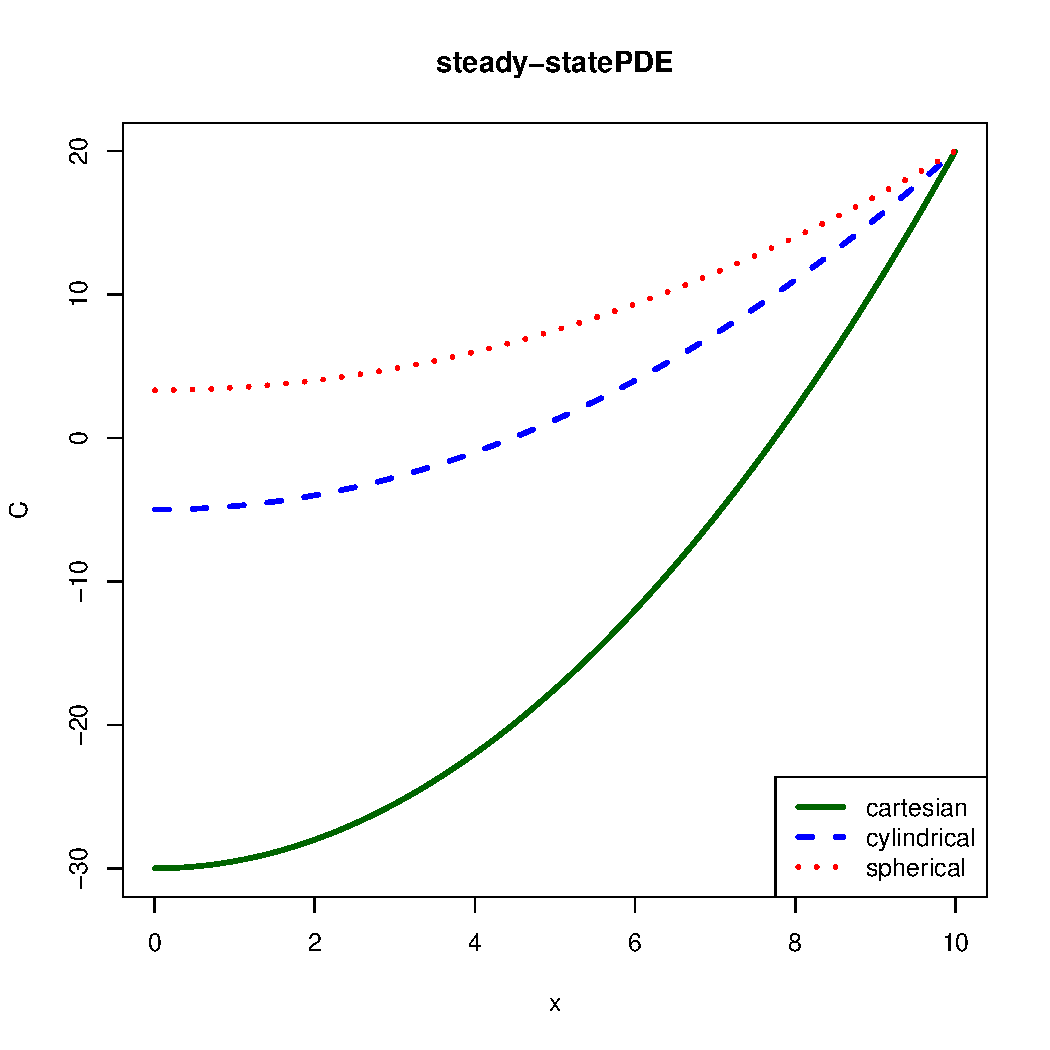
\includegraphics[width=\maxwidth]{figure/unnamed-chunk-14-1} 
\end{knitrout}

\subsection{asdfasdf}

\begin{knitrout}
\definecolor{shadecolor}{rgb}{0.969, 0.969, 0.969}\color{fgcolor}\begin{kframe}
\begin{alltt}
\hlstd{times}\hlkwb{<-}\hlkwd{seq}\hlstd{(}\hlnum{0}\hlstd{,}\hlnum{100}\hlstd{,}\hlkwc{by}\hlstd{=}\hlnum{1}\hlstd{)}

\hlkwd{system.time}\hlstd{(}
  \hlstd{out}\hlkwb{<-}\hlkwd{ode.1D}\hlstd{(}\hlkwc{y}\hlstd{=}\hlkwd{rep}\hlstd{(}\hlnum{1}\hlstd{,Grid}\hlopt{$}\hlstd{N),}\hlkwc{times}\hlstd{=times,}\hlkwc{func}\hlstd{=pde1D,} \hlkwc{parms}\hlstd{=}\hlkwa{NULL}\hlstd{,}\hlkwc{nspec}\hlstd{=}\hlnum{1}\hlstd{,}\hlkwc{A}\hlstd{=r2)}
  \hlstd{)}
\end{alltt}
\begin{verbatim}
##    user  system elapsed 
##   0.157   0.008   0.165
\end{verbatim}
\begin{alltt}
\hlkwd{tail}\hlstd{(out[,}\hlnum{1}\hlopt{:}\hlnum{4}\hlstd{],}\hlkwc{n}\hlstd{=}\hlnum{3}\hlstd{)}
\end{alltt}
\begin{verbatim}
##        time        1        2        3
##  [99,]   98 3.332278 3.332303 3.332366
## [100,]   99 3.332383 3.332408 3.332471
## [101,]  100 3.332478 3.332503 3.332566
\end{verbatim}
\begin{alltt}
\hlkwd{image}\hlstd{(out,}\hlkwc{grid}\hlstd{=Grid}\hlopt{$}\hlstd{x.mid,}\hlkwc{xlab}\hlstd{=}\hlstr{"time,days"}\hlstd{,} \hlkwc{ylab}\hlstd{=}\hlstr{"Distance,cm"}\hlstd{,}\hlkwc{main}\hlstd{=}\hlstr{"PDE"}\hlstd{,}\hlkwc{add.contour}\hlstd{=}\hlnum{TRUE}\hlstd{)}
\end{alltt}
\end{kframe}
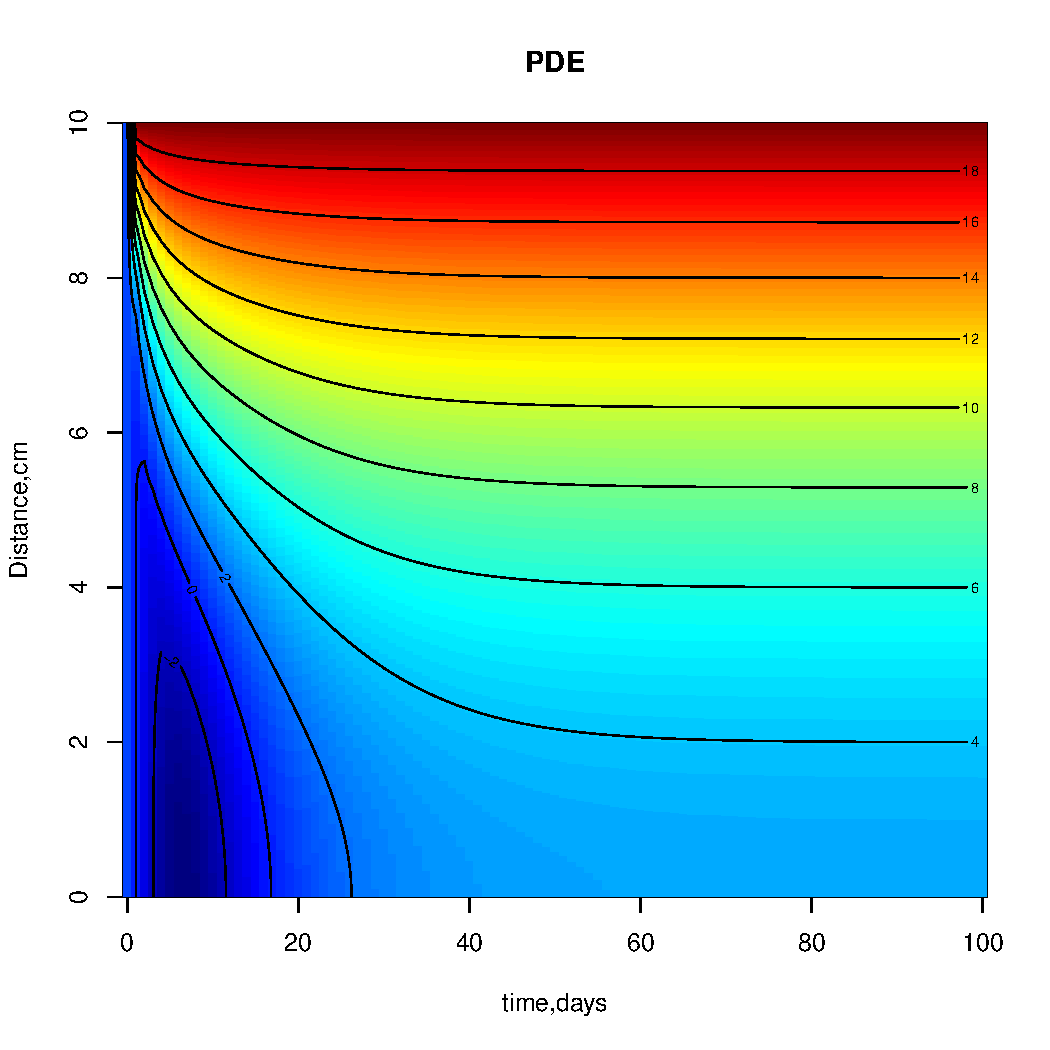
\includegraphics[width=\maxwidth]{figure/unnamed-chunk-15-1} 
\end{knitrout}


\subsection{Oxygen Consumption Porous Spherical Particle}



%\printclassoptions

% Setting up the margins, etc for R


\subsection{2 dimensional diffusion}


\begin{knitrout}
\definecolor{shadecolor}{rgb}{0.969, 0.969, 0.969}\color{fgcolor}\begin{kframe}
\begin{alltt}
\hlstd{diffusion2D} \hlkwb{<-} \hlkwa{function}\hlstd{(}\hlkwc{t}\hlstd{,}\hlkwc{conc}\hlstd{,}\hlkwc{par}\hlstd{)\{}
\hlstd{Conc} \hlkwb{<-} \hlkwd{matrix}\hlstd{(}\hlkwc{nr}\hlstd{=n,}\hlkwc{nc}\hlstd{=n,}\hlkwc{data}\hlstd{=conc)} \hlcom{# vector to 2-D matrix}
\hlstd{dConc} \hlkwb{<-} \hlopt{-}\hlstd{r}\hlopt{*}\hlstd{Conc}\hlopt{*}\hlstd{Conc} \hlcom{# consumption}
\hlstd{BND} \hlkwb{<-} \hlkwd{rep}\hlstd{(}\hlnum{1}\hlstd{,n)} \hlcom{# boundary concentration}

\hlcom{# constant production in certain cells}
\hlstd{dConc[ii]}\hlkwb{<-} \hlstd{dConc[ii]}\hlopt{+} \hlstd{p}

\hlcom{#diffusion in X-direction; boundaries=imposed concentration}

\hlstd{Flux} \hlkwb{<-} \hlopt{-}\hlstd{Dx} \hlopt{*} \hlkwd{rbind}\hlstd{(}\hlkwd{rep}\hlstd{(}\hlnum{0}\hlstd{,n),(Conc[}\hlnum{2}\hlopt{:}\hlstd{n,]}\hlopt{-}\hlstd{Conc[}\hlnum{1}\hlopt{:}\hlstd{(n}\hlopt{-}\hlnum{1}\hlstd{),]),}\hlkwd{rep}\hlstd{(}\hlnum{0}\hlstd{,n))}\hlopt{/}\hlstd{dx}
\hlstd{dConc} \hlkwb{<-} \hlstd{dConc} \hlopt{-} \hlstd{(Flux[}\hlnum{2}\hlopt{:}\hlstd{(n}\hlopt{+}\hlnum{1}\hlstd{),]}\hlopt{-}\hlstd{Flux[}\hlnum{1}\hlopt{:}\hlstd{n,])}\hlopt{/}\hlstd{dx}

\hlcom{#diffusion in Y-direction}
\hlstd{Flux} \hlkwb{<-} \hlopt{-}\hlstd{Dy} \hlopt{*} \hlkwd{cbind}\hlstd{(}\hlkwd{rep}\hlstd{(}\hlnum{0}\hlstd{,n),(Conc[,}\hlnum{2}\hlopt{:}\hlstd{n]}\hlopt{-}\hlstd{Conc[,}\hlnum{1}\hlopt{:}\hlstd{(n}\hlopt{-}\hlnum{1}\hlstd{)]),}\hlkwd{rep}\hlstd{(}\hlnum{0}\hlstd{,n))}\hlopt{/}\hlstd{dy}
\hlstd{dConc} \hlkwb{<-} \hlstd{dConc} \hlopt{-} \hlstd{(Flux[,}\hlnum{2}\hlopt{:}\hlstd{(n}\hlopt{+}\hlnum{1}\hlstd{)]}\hlopt{-}\hlstd{Flux[,}\hlnum{1}\hlopt{:}\hlstd{n])}\hlopt{/}\hlstd{dy}

\hlkwd{return}\hlstd{(}\hlkwd{list}\hlstd{(}\hlkwd{as.vector}\hlstd{(dConc)))}
\hlstd{\}}
\end{alltt}
\end{kframe}
\end{knitrout}

After specifying the values of the parameters, 10 cells on the 2-D grid where there will be
substance produced are randomly selected (ii).

14 Package rootSolve : roots, gradients and steady-states in R
0.0 0.2 0.4 0.6 0.8 1.0
0.0 0.2 0.4 0.6 0.8 1.0
2-D diffusion+production
x
y
Figure 5: Steady-state solution of the nonlinear 2-Dimensional model
\begin{knitrout}
\definecolor{shadecolor}{rgb}{0.969, 0.969, 0.969}\color{fgcolor}\begin{kframe}
\begin{alltt}
\hlcom{# parameters}
\hlstd{dy} \hlkwb{<-} \hlstd{dx} \hlkwb{<-} \hlnum{1} \hlcom{# grid size}
\hlstd{Dy} \hlkwb{<-} \hlstd{Dx} \hlkwb{<-} \hlnum{1.5} \hlcom{# diffusion coeff, X- and Y-direction}
\hlstd{r} \hlkwb{<-} \hlnum{0.01} \hlcom{# 2-nd-order consumption rate (/time)}
\hlstd{p} \hlkwb{<-} \hlnum{20} \hlcom{# 0-th order production rate (CONC/t)}
\hlstd{n} \hlkwb{<-} \hlnum{100}
\hlcom{# 10 random cells where substance is produced at rate p}
\hlstd{ii} \hlkwb{<-} \hlkwd{trunc}\hlstd{(}\hlkwd{cbind}\hlstd{(}\hlkwd{runif}\hlstd{(}\hlnum{10}\hlstd{)}\hlopt{*}\hlstd{n}\hlopt{+}\hlnum{1}\hlstd{,}\hlkwd{runif}\hlstd{(}\hlnum{10}\hlstd{)}\hlopt{*}\hlstd{n}\hlopt{+}\hlnum{1}\hlstd{))}
\end{alltt}
\end{kframe}
\end{knitrout}
The steady-state is found using function steady.2D. It takes as arguments a.o. the dimensionality
of the problem (dimens) and lrw=1000000, the length of the work array needed by
the solver. If this value is set too small, the solver will return with the size needed.
It takes about 0.5 second to solve this 10000 state variable model.
\begin{knitrout}
\definecolor{shadecolor}{rgb}{0.969, 0.969, 0.969}\color{fgcolor}\begin{kframe}
\begin{alltt}
\hlstd{Conc0} \hlkwb{<-} \hlkwd{matrix}\hlstd{(}\hlkwc{nr}\hlstd{=n,}\hlkwc{nc}\hlstd{=n,}\hlnum{10.}\hlstd{)}
\hlkwd{print}\hlstd{(}\hlkwd{system.time}\hlstd{(}
\hlstd{ST3} \hlkwb{<-} \hlkwd{steady.2D}\hlstd{(Conc0,}\hlkwc{func}\hlstd{=diffusion2D,}\hlkwc{parms}\hlstd{=}\hlkwa{NULL}\hlstd{,}\hlkwc{pos}\hlstd{=}\hlnum{TRUE}\hlstd{,}\hlkwc{dimens}\hlstd{=}\hlkwd{c}\hlstd{(n,n),}
\hlkwc{lrw}\hlstd{=}\hlnum{1000000}\hlstd{,}\hlkwc{atol}\hlstd{=}\hlnum{1e-10}\hlstd{,}\hlkwc{rtol}\hlstd{=}\hlnum{1e-10}\hlstd{,}\hlkwc{ctol}\hlstd{=}\hlnum{1e-10}\hlstd{)}
\hlstd{))}
\end{alltt}
\begin{verbatim}
##    user  system elapsed 
##   0.224   0.005   0.230
\end{verbatim}
\end{kframe}
\end{knitrout}
user system elapsed
1.044 0.032 1.076
The S3 image method is used to generate the steady-state plot.

\begin{knitrout}
\definecolor{shadecolor}{rgb}{0.969, 0.969, 0.969}\color{fgcolor}\begin{kframe}
\begin{alltt}
\hlkwd{image}\hlstd{(ST3,}\hlkwc{main}\hlstd{=}\hlstr{"2-D diffusion+production"}\hlstd{,} \hlkwc{xlab}\hlstd{=}\hlstr{"x"}\hlstd{,} \hlkwc{ylab}\hlstd{=}\hlstr{"y"}\hlstd{)}
\end{alltt}
\end{kframe}
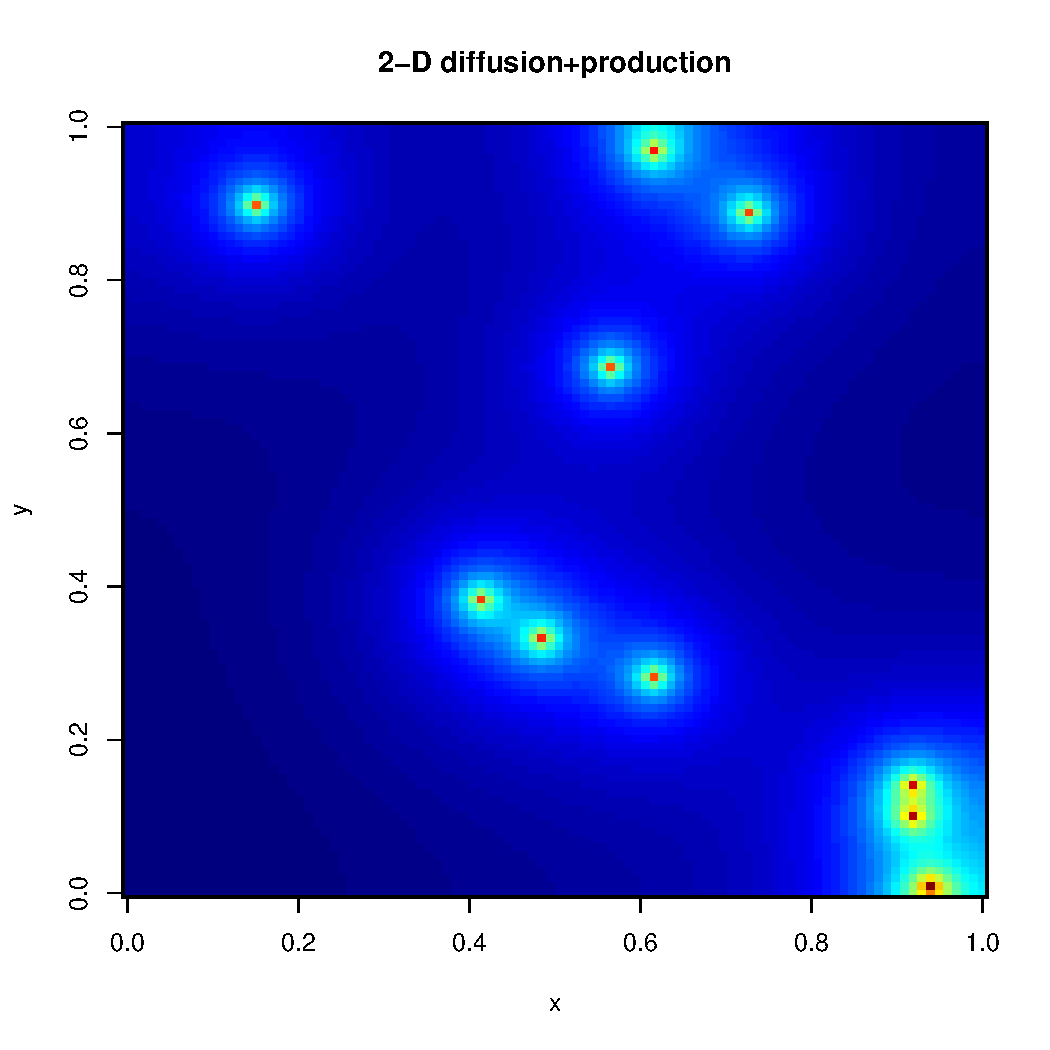
\includegraphics[width=\maxwidth]{figure/unnamed-chunk-19-1} 
\end{knitrout}

\begin{knitrout}
\definecolor{shadecolor}{rgb}{0.969, 0.969, 0.969}\color{fgcolor}\begin{kframe}
\begin{alltt}
\hlstd{pde2D} \hlkwb{<-} \hlkwa{function} \hlstd{(}\hlkwc{t}\hlstd{,} \hlkwc{y}\hlstd{,} \hlkwc{parms}\hlstd{) \{}
\hlstd{CONC} \hlkwb{<-} \hlkwd{matrix}\hlstd{(}\hlkwc{nr} \hlstd{= n,} \hlkwc{nc} \hlstd{= n, y)}
\hlstd{Tran} \hlkwb{<-} \hlkwd{tran.2D}\hlstd{(CONC,} \hlkwc{D.x} \hlstd{= Dx,} \hlkwc{D.y} \hlstd{= Dy,} \hlkwc{dx} \hlstd{= dx,} \hlkwc{dy} \hlstd{= dy)}
\hlstd{dCONC} \hlkwb{<-} \hlstd{Tran}\hlopt{$}\hlstd{dC} \hlopt{-} \hlstd{r} \hlopt{*} \hlstd{CONC}
\hlstd{dCONC[ii]}\hlkwb{<-} \hlstd{dCONC[ii]} \hlopt{+} \hlstd{p}
\hlkwd{return}\hlstd{(}\hlkwd{list}\hlstd{(}\hlkwd{as.vector}\hlstd{(dCONC)))}
\hlstd{\}}
\end{alltt}
\end{kframe}
\end{knitrout}

Before running the model, the grid sizes (dx, dx), diffusion coefficients (Dx, Dy), 1st order
consumption rate (r) are defined. There are 100 boxes in x- and y direction (n). Furthermore,
we assume that the substance is produced in 50 randomly chosen cells (ii) at a constant rate
(p):

\begin{knitrout}
\definecolor{shadecolor}{rgb}{0.969, 0.969, 0.969}\color{fgcolor}\begin{kframe}
\begin{alltt}
\hlstd{n} \hlkwb{<-} \hlnum{100}
\hlstd{dy} \hlkwb{<-} \hlstd{dx} \hlkwb{<-} \hlnum{1}
\hlstd{Dy} \hlkwb{<-} \hlstd{Dx} \hlkwb{<-} \hlnum{2}
\hlstd{r} \hlkwb{<-} \hlnum{0.001}
\hlstd{p} \hlkwb{<-} \hlkwd{runif}\hlstd{(}\hlnum{50}\hlstd{)}
\hlstd{ii} \hlkwb{<-} \hlkwd{trunc}\hlstd{(}\hlkwd{cbind}\hlstd{(}\hlkwd{runif}\hlstd{(}\hlnum{50}\hlstd{)} \hlopt{*} \hlstd{n,} \hlkwd{runif}\hlstd{(}\hlnum{50}\hlstd{)} \hlopt{*} \hlstd{n)} \hlopt{+} \hlnum{1}\hlstd{)}
\end{alltt}
\end{kframe}
\end{knitrout}

\begin{knitrout}
\definecolor{shadecolor}{rgb}{0.969, 0.969, 0.969}\color{fgcolor}\begin{kframe}
\begin{alltt}
\hlstd{Conc0} \hlkwb{<-} \hlkwd{matrix}\hlstd{(}\hlkwc{nr} \hlstd{= n,} \hlkwc{nc} \hlstd{= n,} \hlnum{10}\hlstd{)}
\hlkwd{print}\hlstd{(}\hlkwd{system.time}\hlstd{(ST} \hlkwb{<-} \hlkwd{steady.2D}\hlstd{(}\hlkwc{y} \hlstd{= Conc0,} \hlkwc{func} \hlstd{= pde2D,}
\hlkwc{parms} \hlstd{=} \hlkwa{NULL}\hlstd{,} \hlkwc{dimens} \hlstd{=} \hlkwd{c}\hlstd{(n, n),} \hlkwc{lrw} \hlstd{=} \hlnum{6e+05}\hlstd{)))}
\end{alltt}
\begin{verbatim}
##    user  system elapsed 
##   0.067   0.005   0.072
\end{verbatim}
\end{kframe}
\end{knitrout}

\begin{knitrout}
\definecolor{shadecolor}{rgb}{0.969, 0.969, 0.969}\color{fgcolor}\begin{kframe}
\begin{alltt}
\hlkwd{image}\hlstd{(ST,} \hlkwc{main} \hlstd{=} \hlstr{"steady-state 2-D PDE"}\hlstd{)}
\end{alltt}
\end{kframe}
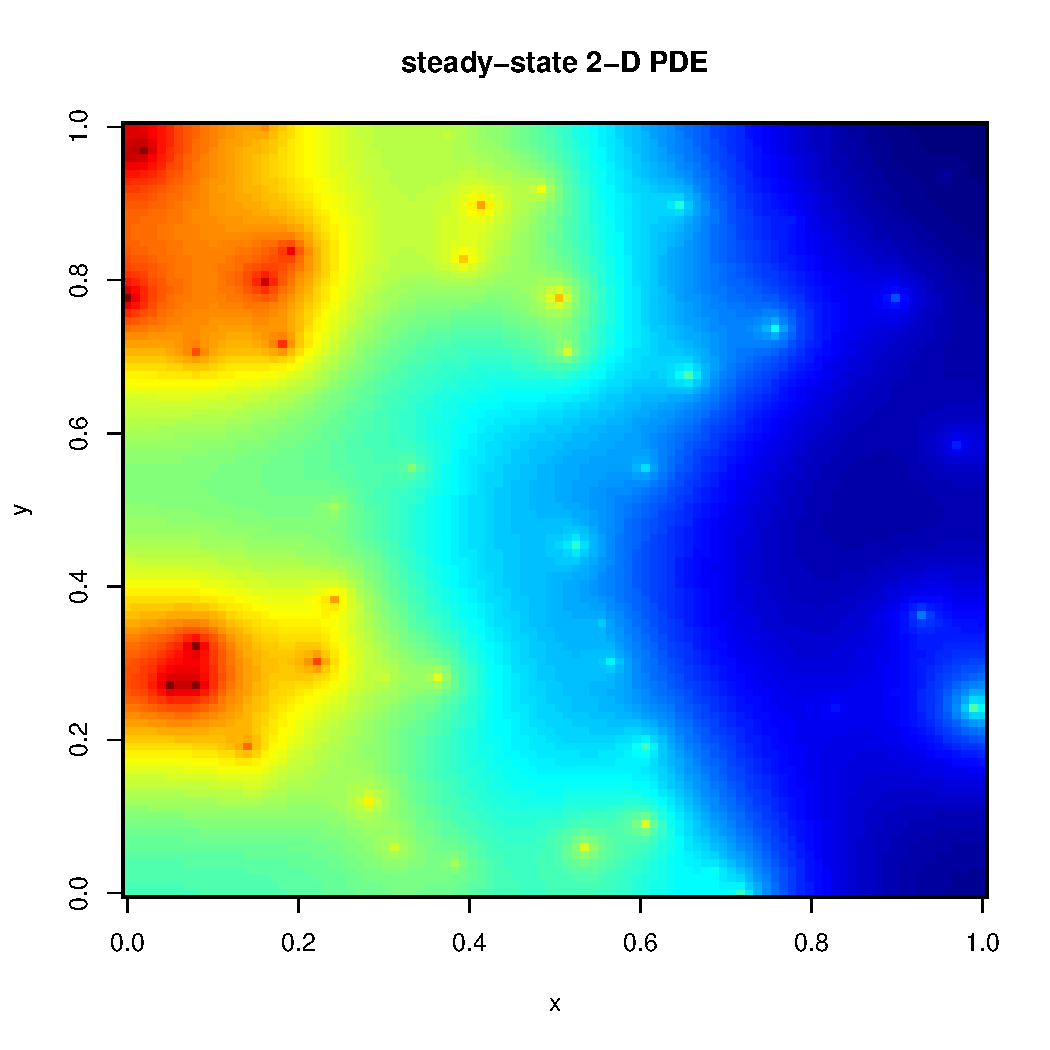
\includegraphics[width=\maxwidth]{figure/unnamed-chunk-23-1} 
\end{knitrout}


\section{Considering 2D Models}

2.4. Steady-state solution of 2-D PDEs
Function steady.2D effciently snds the steady-state of 2-dimensional problems.
Karline Soetaert 13
In the following model
@C
@t
= Dx 
@2C
@x2 + Dy 
@2C
@y2
.. r  C2 + pxy
a substance C is consumed at a quadratic rate (r C2), while dispersing in X- and Y-direction.
At certain positions (x,y) the substance is produced (rate p).
The model is solved on a square (100*100) grid. There are zero-
ux boundary conditions at
the 4 boundaries.
The term Dx  @2C
@x2 is in fact shorthand for:
..
@Flux
@x
where
Flux = ..Dx 
@C
@x
i.e. it is the negative of the 
ux gradient, where the 
ux is due to diffusion.
In the numerical approximation fo the 
ux, the concentration gradient is approximated as the
subtraction of two matrices, with the columns or rows shifted (e.g. Conc[2:n,]-Conc[1:(n-1),]).
The 
ux gradient is then also approximated by subtracting entire matrices
(e.g. Flux[2:(n+1),]-Flux[1:(n),]). This is very fast. The zero-
ux at the boundaries is
imposed by binding a column or row with 0-s.


\section{The Theory}

\subsection{Advection and Convection: Material and Heat}

Advection is the transport of a substance by bulk motion. Convection is the transfer of heat by the actual movement of the warmed matter. The equation that are used to describe advection and convection are similar, but the physical processes are different.

\subsection{Solving the advection-diffusion equation}

The advection-diffusion equation is a partial differential equation that describes the transport of a substance by both diffusion and advection.

\subsecton{Goals of these notes}

\begin{itemize}

\item Introduce the advection-diffusion equation
\item Find solution for steady-state XX transfer with a constant XX flux
\item Find solution for steady-state solute transfer with a constant basal??

\end{itemize}

\subsection{Advection-diffusion equation in 1D}

To show how the advection equation can be solved, we're actually going to look at a combination of the advection and diffusion equations applied to compound advection and diffusion.

transfer equations in 1D, with math that is straightforward to follow.

Disperson is a diffusion process caused by interactions of atoms or molecules, which can be simulated using the diffusion equation we saw in last week's notes.

Mathematically, we'll start with our two equations: (1) The diffusion equation without heat production and (2) the advection equation, then combine them.

\begin{equation}
    \frac{\partial T}{\partial t} &= \kappa \frac{\partial^{2} T}{\partial z^{2}} ~~ \text{Diffusion}\\
\end{equation}

\begin{equation}
    \frac{\partial T}{\partial t} &= v_{z}\frac{\partial T}{\partial z} ~~ \text{Advection}\\
\end{equation}    
\begin{equation}
    \frac{\partial T}{\partial t} &= \kappa \frac{\partial^{2} T}{\partial z^{2}} + v_{z}\frac{\partial T}{\partial z} ~~ \text{Diffusion + Advection}
\end{equation}

In steady state, we can ignore the transient term $\partial T/\partial t$, so

\begin{equation}
    \cancel{\frac{\partial T}{\partial t}}{\frac{\partial T}{\partial t}} &= \kappa \frac{\partial^{2} T}{\partial z^{2}} + v_{z}\frac{\partial T}{\partial z} ~~ \text{ Steady-state advection-diffusion equation}\\
    
\end{equation}    
\begin{equation}

    \frac{\partial^{2} T}{\partial z^{2}} &= -\frac{v_{z}}{\kappa} \frac{\partial T}{\partial z} ~~ \text{ Rearranged}\\
    
    \end{equation}

Another way to write the previous equation is

\begin{equation}
    \frac{\partial}{\partial z} \left(\frac{\partial T}{\partial z}\right) = -\frac{v_{z}}{\kappa} \frac{\partial T}{\partial z}
    
    \end{equation}

In this case, we can make some substitutions and find something quite useful.
Assume $f = \partial T/\partial z$ and $c = v_{z}/\kappa$.
With this, we can say $f'(z) = -c f(z)$ .


This is a common form of differential equation with a solution $f(z) = f(0) \mathrm{e}^{cz}$ .
Thus, in terms of our equation we can say

\begin{equation}

    \frac{\partial T}{\partial z} = \left. -\frac{\partial T}{\partial z} \right|_{(z = 0)} \mathrm{e}^{-(v_{z} z/\kappa)}
    
    \end{equation}

\subsection{Solutions to the steady-state advection-diffusion equation}

The simplest solution to the previous equation is to assume a constant temperature gradient 
\begin{equation}
    \frac{\partial T}{\partial z} &= \left. -\frac{\partial T}{\partial z} \right|_{(z = 0)} \mathrm{e}^{-(v_{z} z/\kappa)} = g \mathrm{e}^{-(v_{z} z/\kappa)}\\
 \end{equation}    
\begin{equation}   
    
    \int \frac{\partial T}{\partial z} &= g \int \mathrm{e}^{-(v_{z} z/\kappa)} && \text{Integrate}\\
    T(z) &= -\frac{g \kappa}{v_{z}} \mathrm{e}^{-(v_{z} z/\kappa)} + c_{1}
    \end{equation}

Assume $T(0) = 0$.

\begin{equation}

    T(z) &= -\frac{g \kappa}{v_{z}} \mathrm{e}^{-(v_{z} z/\kappa)} + c_{1}\\
  \end{equation}    
\begin{equation}  
    0 &= -\frac{g \kappa}{v_{z}} \cancelto{1}{\mathrm{e}^{-(v_{z} 0/\kappa)}} + c_{1}\\
    c_{1} &= \frac{g \kappa}{v_{z}}
    
\end{equation}

Thus, we find

\begin{equation}

    T(z) &= -\frac{g \kappa}{v_{z}} \mathrm{e}^{-(v_{z} z/\kappa)} + \frac{g \kappa}{v_{z}}\\
 \end{equation}    
\begin{equation}   
    T(z) &= \frac{g \kappa}{v_{z}}\left(1 - \mathrm{e}^{-(v_{z} z/\kappa)} \right) ~~\text{Rearranged}

    What should our temperature profile look like?

    At constant $z$ , what happens to $T$ if $v_{z}$ gets large?

Constant temperature $T_{L}$ at $z=L$

A more useful second boundary condition is to assume $T(L) = T_{L}$.
In this case

\begin{equation}

    T(z) = T_{L} \left( \frac{1 - \mathrm{e}^{-(v_z z / \kappa})}{1 - \mathrm{e}^{-(v_z L / \kappa})} \right)
\end{equation}


%\subsecton{The Peclet number}

%The Peclet number is a useful value for estimating the relative influence of advective versus diffusive heat transfer processes.

%\begin{equation}
%    \mathrm{Pe} = \frac{v_{z}L}{\kappa}
%\end{equation}

%Where $\kappa$` is a parameter known as the *thermal diffusivity*.

%$\kappa$ is the rock thermal conductivity $k$ divided by the product of the density $\rho$ and heat capacity $c_{\mathrm{p}}$, or $\kappa = k / (\rho c_{\mathrm{p}})$.

%If a typical rock thermal diffusivity is $\kappa = 10^{-6}$ and typical continental crust is 35 km thick, how fast does it need to erode for advection exceed the effects of diffusion?

%How would this be different for erosion of the entire lithosphere?

\subsection{Advection-diffusion equation take-home messages}

\begin{itemize*}

    \item Math gets a bit more complex, even for the 'simplest' cases; Often need numerical methods for more complex geometries

    \item Behavior of the equation is strongly controlled by the boundary conditions

    \item Even these simple equations can be quite useful. Advection can be a significant influence on the thermal field and these simple calculations allow you to estimate when it is a factor and its magnitude of influence.
\end{itemize*}


Some Caveats:

\begin{itemize*}
  \item Steady-state
  \item 1-D
  \item Constants assumed to be constant :)
  \item No heat production
  
\end{itemize*}


\section{Conclusion}

\end{comment}

\newpage

\section{References}

% bibiliography section here-------------------------------------------
%\clearpage

\url{https://en.wikipedia.org/wiki/Convection%E2%80%93diffusion_equation}



\bibliographystyle{apalike}
%\renewcommand\bibname{References}{}
\bibliography{/home/mwl04747/RTricks/references}%	\addcontentsline{toc}{chapter}{References}


\end{document}
